%% jnuthesis 文档类的可选参数有:
%%   nobackinfo 取消封二页导师签名信息.注意,按照南大的规定,是需要签名页的.
%%   phd/master/bachelor 选择博士/硕士/学士论文

% 使用 blindtext 宏包自动生成章节文字
% 这仅仅是用于生成样例文档,正式论文中一般用不到该宏包
\documentclass[bachelor,adobefonts]{jnuthesis}

% 本科课程设计课程名称
\usepackage{graphicx}
\usepackage{subcaption}
\usepackage{algorithm}
\usepackage{algorithmic} 
\usepackage{amsmath}  
 
\renewcommand{\algorithmicrequire}{\textbf{Input:}} 
\renewcommand{\algorithmicensure}{\textbf{Output:}}


\graphicspath{ {images/} }
%%%%%%%%%%%%%%%%%%%%%%%%%%%%%%%%%%%%%%%%%%%%%%%%%%%%%%%%%%%%%%%%%%%%%%%%%%%%%%%
% 设置论文的中文封面

% 如果论文标题过长,可以分两行,第一行用\titlea{}定义,第二行用\titleb{}定义,将上面的\title{}注释掉
\titlea{复杂网络技术在数据挖掘中的应}
\titleb{用}



% 论文作者姓名
\author{汪建海}
% 论文作者学生证号
\studentnum{1030414623}
% 导师姓名职称
\supervisor{方伟}
\supervisorpos{讲师}
% 第二行导师姓名职称,仿照第一行填写,没有则留空
\supervisorb{}
\supervisorbpos{}
% 论文作者的学科与专业方向
\major{计算机科学与技术}
% 论文作者所在院系的中文名称,学士学位论文此处不带“学院”二字
\department{物联网工程}
% 论文作者所在学校或机构的名称.此属性可选,默认值为``江南大学''.
\institute{江南大学}
% 学士学位获得日期,需设置年、月,默认为编译日期.
\bachelordegreeyear{2018}
\bachelordegreemonth{6}
%%%%%%%%%%%%%%%%%%%%%%%%%%%%%%%%%%%%%%%%%%%%%%%%%%%%%%%%%%%%%%%%%%%%%%%%%%%%%%%

%-------------------------------------------------------------------------------
%	CODE INCLUSION CONFIGURATION
%-------------------------------------------------------------------------------
\usepackage{listings}
\newfontfamily\menlo{Menlo}
\usepackage{color}
\lstset{
    columns=fixed,
    breaklines=true,
    numbers=left,                                        % 在左侧显示行号
    frame=single,                                        % 显示背景边框
    % backgroundcolor=\color[RGB]{245,245,244},            % 设定背景颜色
    % keywordstyle=\color[RGB]{40,40,255},                 % 设定关键字颜色
    numberstyle=\footnotesize\color{darkgray},           % 设定行号格式
    % commentstyle=\color[RGB]{0,96,96},                   % 设置代码注释的格式
    % stringstyle=\color[RGB]{128,0,0},                    % 设置字符串格式
    showstringspaces=false,                              % 不显示字符串中的空格
    basicstyle=\small\menlo,
    numberstyle=\scriptsize\menlo,
    xleftmargin=0cm,
    xrightmargin=0cm
}

\begin{document}

%%%%%%%%%%%%%%%%%%%%%%%%%%%%%%%%%%%%%%%%%%%%%%%%%%%%%%%%%%%%%%%%%%%%%%%%%%%%%%%

% 制作中文封面
\maketitle

%%%%%%%%%%%%%%%%%%%%%%%%%%%%%%%%%%%%%%%%%%%%%%%%%%%%%%%%%%%%%%%%%%%%%%%%%%%%%%%
% % 开始前言部分
% \frontmatter

%%%%%%%%%%%%%%%%%%%%%%%%%%%%%%%%%%%%%%%%%%%%%%%%%%%%%%%%%%%%%%%%%%%%%%%%%%%%%%%
% 论文的中文摘要
\begin{abstract}

自然语言理解是自然语言处理乃至人工智能领域亟待研究重点与难点,
对其研究在理论上和实际应用上都有重要的意义.
随着深度学习的发展,基于循环神经网络(RNN)、长短期记忆网络(LSTM)等的序列建模方式已经成为了
自然语言处理的主流方法.
但是这些深度学习模型需要大规模训练数据,并且将复杂的语言分析和理解
过程简化成“黑盒子”,难以融合先验语言知识,进而使模型缺乏可解释性.

本文尝试将先验文本语言学知识引入传统深度学习模型中,提出了融合句法结构的深度神经网络.
该模型通过依存句法分析工具获得文本的句法子结构,
然后将文本的语义表示和结构表示分别通过两个独立的LSTM模型,
再将子结构输出的加权平均结果与主文本句子的输出结果相融合,
从而实现利用句法结构信息对句子表示增强,最后将这个增强表示送入后续的神经网络中以完成文本分类、机器翻译等文本理解应用.

通过在文本理解的基础性任务文本分类上进行对照实验,
得出融合模型相对传统深度学习模型具有以下两个主要优点:
(1)由于引入了语言学知识,在小规模数据集上有明显优势;在大规模数据集上也有一定优势,模型有较好的鲁棒性.
(2)通过Attention机制可视化文本中不同结构的重要程度,使得模型具有一定的可解释性.

在实验中还对融合模型的Attention机制和融合方式开展了进一步的研究.最终在AGNews数据集上,
融合模型相对于LSTM模型在测试集上的正确率提升了2.5\%.

% 中文关键词.关键词之间用中文全角分号隔开,末尾无标点符号.
\keywords{文本理解;依存句法结构;深度学习 ;融合模型}
\end{abstract}

%%%%%%%%%%%%%%%%%%%%%%%%%%%%%%%%%%%%%%%%%%%%%%%%%%%%%%%%%%%%%%%%%%%%%%%%%%%%%%%
% 论文的英文摘要



\begin{englishabstract}
Natural language understanding is an urgent task in the field of natural language processing and artificial intelligence.
The research is of great significance in both theory and practice.
In recent years, with the development of deep learning, the sequential modeling methods based on Recurrent Neural Network (RNN) and Long Short Term Memory Network (LSTM) have been established.
The mainstream method of natural language processing.
But these deep learning models require massive training of data and complex language analysis and understanding.
The process is simplified into “black box”, which is difficult to combine with the prior language knowledge, thus making the model lack of interpretability.
  
This paper attempts to introduce the knowledge of prior text linguistics into the traditional deep learning model, and puts forward the deep neural network of syntactic structure.
This model acquires the syntactic substructure of text by means of the dependency syntactic analysis tool.
Then the semantic representation and structure of the text are represented by two separate LSTM models.
The weighted average result of the substructure output is combined with the output result of the main text sentence.
In this way, the sentence is enhanced by using syntactic structure information. Finally, this enhancement is sent to the subsequent neural network to complete the application of text classification, machine translation and other text understanding.
  
By conducting a controlled experiment on the basic task text categorization of text comprehension,
It is concluded that the fusion model has two main advantages:
(1) due to the introduction of linguistic knowledge, there are obvious advantages in the small-scale data set; There are some advantages in large-scale data sets, and the model has good robustness.
(2) the importance of different structures in the visual text of the Attention mechanism makes the model have certain interpretability.
  
In the experiment, the Attention mechanism and fusion mode of the fusion model were further studied. Finally, in the AGNews data set,
The accuracy of the fusion model in the test set was increased by 2.5\% compared with the LSTM model.
% 英文关键词.关键词之间用英文半角逗号隔开,末尾无符号.
\englishkeywords{Text understanding;Structure of dependency syntax; Deep learning; Fusion model}
\end{englishabstract}

%%%%%%%%%%%%%%%%%%%%%%%%%%%%%%%%%%%%%%%%%%%%%%%%%%%%%%%%%%%%%%%%%%%%%%%%%%%%%%%
% 生成论文目次
\tableofcontents

%%%%%%%%%%%%%%%%%%%%%%%%%%%%%%%%%%%%%%%%%%%%%%%%%%%%%%%%%%%%%%%%%%%%%%%%%%%%%%%
% 开始正文部分
\mainmatter

%%%%%%%%%%%%%%%%%%%%%%%%%%%%%%%%%%%%%%%%%%%%%%%%%%%%%%%%%%%%%%%%%%%%%%%%%%%%%%%
% 学位论文的正文应以《绪论》作为第一章

%第一章绪论
\chapter{绪论}\label{chapter_introduction}
\section{选题背景与意义}
数据挖掘(Data Mining,DM)又称数据库中的知识发现(Knowledge Discover in DataBase,KDD),
涉及了机器学习、人工智能、数据库理论以及统计学等学科的交叉研究领域.
数据挖掘就是从数据库中的大量数据中挖掘有效的信息,即从不完全的、模糊的、大量的、随机的
实际数据中,去发现有规律的、隐含的、有用的、人们事先未知的但却潜在有价值的并且最终可理解的信息和知识的非平凡过程.

数据挖掘是一种决策支持的过程,它主要基于人工智能、机器学习、模式识别、统计学、数据库、可视化技术等,
高度自动化第分析企业的数据,做出归纳性的推理,从中挖掘出潜在的模式,
帮助决策者调整市场策略,减少风险,做出正确的决策.

所以对挖掘技术的研究必然可以提高游泳信息的获取,
从而直接或间接推动这些应用的性能和实用性的提高,具有重要的研究意义和价值.

\section{数据挖掘的发展与现状}
\subsection{数据挖掘的历史及发展}

数据挖掘的发展是建立在相关学科发展的基础上.
随着数据库技术的发展及数据的应用,人们积累的数据越来越多.
激增的数据背后面隐藏很多重要信息,简单的查询和统计已经无法满足商业需求,
需要一种挖掘数据背后隐藏知识的手段.

同时人工智能(Artificial Intelligence,AI)自1956年诞生以来就取得了重大进展.
经历了博弈时期、自然语言理解、知识工程等阶段,目前的热点是机器学习.
用数据库管理系统来存储数据,用机器学习的方法来分析数据,挖掘大量数据背后的知识,
这两者的结合促成了数据库中的知识发现(Knowledge Discover in DataBase,KDD)的产生.

1989年8月在美国底特律召开了第十一届人工智能联合会议的专题讨论会上首次出现了知识发现(KDD)这个术语.
1998年在第四届知识发现与数据挖掘国际学术会议上不仅进行了学术讨论,
而且有30多家软件公司展示了他们数据挖掘的产品,不少软件在北美和欧洲得到了广泛的应用.
数据挖掘经历十多年的发展,现在已经成为了一个自成体系的学科.

进入20世纪70年代后期,在数据挖掘取得了两大成就:

(1)广义线性模型.
广义选型建模是线性模型在研究响应值的正态分布以及非线性模型的简介直接的线性转化时的一种发展.
其最大作用就是将零碎的统计研究的多方面贡献统一起来,概括了基于正态理论以外的线性模型的研究.

(2)EM算法.
EM算法是Dempster Laind Rubin于1977年提出的一种求参数极大似然估计的方法,
它可以从非完整数据集中对参数进行MLE估计,应用于处理缺损数据,截尾数据,带有噪声等所谓不完整数据(Incomplete Data),
起重要作用是解决不完整数据估计问题的数值问题.

20世纪80年代以后,资料模拟及非参统计的发展使得数据挖掘技术进入崭新的阶段,SVM、神经网络、Bootsrap法的提出,
以及处理变量非线性关系的核光滑(Kernel Smoothing)法增强了数据挖掘的识别能力.

从20世纪70年代,数据挖掘技术主要经历了四个阶段,总结如图(1-1)所示:

\begin{figure}[htp]
  \centering
  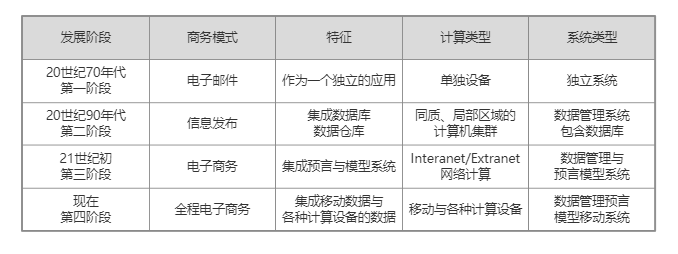
\includegraphics[width=1.0\linewidth]{Wsjwj.png}
  \caption{数据挖掘发展}
\end{figure}


\subsection{数据挖掘的研究现状}
目前我国在数据挖掘技术研究上已经取得了巨大的成果,
常用的数据挖掘模型包括神经网络模型、决策树模型、遗传算法模型、粗糙集模型、模糊集模型、关联规则模型等.

(1)神经网络模型基于仿生学理论,模拟生物神经系统和其他操作模式,训练人工智能来学习非线性预测. 
神经网络模型可以实现数据聚合和数据分类等多种功能,其关键在于对权值进行修改,
该模型具有较强的抗干扰和非线性学习能力,可以准确地挖掘复杂的目标,但很难处理高风险变量.

(2)决策树模型可用于通过一系列规则对数据进行分类,其模型结构与程序树结构相似.
模型结构简单而且数据挖掘效率高,但不适合于挖掘多维变量数据.

(3)遗传算法模通过遗传整合、遗传变异,遗传交叉和自然选择等方法实现机器学习过程,
该模型可以处理多种数据类型,但需要设置的参数非常大,建立模型难度大;

(4)粗糙集模型能够处理模糊和不准确的数学问题,但难以处理属性的延续,
并且在数据处理之前属性必须离散化.

(5)模糊集模型可用于模糊识别,模糊分析和数据问题的模糊分类. 
模糊评估,模型越复杂,其数据处理的模糊性越强;

(6)关联规则模型依赖于数据与数据之间的相关性,最典型的关联规则模型是Apriori模型,
该模型可以作为源关联规则,满足数据库中最小支持度和最小信任度 用于通过关联规则挖掘数据.


\section{论文主要工作}
本文围绕研究将数据挖掘中的聚类知识与复杂网络有关模型进行有机融合,提出了基于复杂网络的数据挖掘的应用,
并就特定的用户数据进行研究,本文的主要工作有下面几个方面.

(1)通过查找文献了解复杂网络和数据挖掘的定义和具体实现方法,对现有相关研究做一定的综述工作.

(2)研究知乎用户数据并采用特定的方法对数据进行爬取,并提出有效数据.

(3)通过研究特定的聚类算法并实现,分析实习的效果并分析他的优缺点,进一步改进算法.

(4)用研究的聚类算法并结合复杂网络模型对数据进行分析,通过计算用户间关系相异度,对数据进行分析,
得出数据关系聚类图,分析方法的实际效果

\section{论文结构安排}
本论文总共分为五个章节,每个章节的内容概括如下:

(1)第一章为绪论,首先介绍了课题的研究背景,然后介绍了该领域的研究发展和现状,
并且简单描述了本文的研究内容,最后给出了全文的结构安排.

(2)第二章对复杂网络的相关知识进行详细的说明,并研究论文相关的模型.

(3)第三章介绍数据抓取的细节,并对数据做出一些清洗,为后文提供相应的数据分析.

(4)第四章为聚类算法的研究,详细说明了算法的实现的具体细节并分析实现效果,说明了算法的优缺点,
并对算法的缺点进行适当的改进.

(5)第五章为结论与展望,对本文主要工作进行了总结,对存在的不足进行了展望.





\chapter{复杂网络}
在现实生活中,我们经常发现你的朋友的朋友也是你的朋友,
这一现象就是网络中就是一个节点的几个邻居节点中,有些节点但之间相互也是邻居.
现实生活中很多网络表现除了很强的聚类性,特别式社会网络.
所以本章节主要介绍有关复杂网络的基本理论和相关知识,为后面章节打下了坚实的理论基础.

\section{复杂网络的定义}
所谓的复杂网络就是具有复杂的拓扑结构和动力学行为的大规模网络,
它是由大量的节点通过边的相互连接而构成的图,其中的节点可以是任意具有特定动力和信息
内涵的系统的基本单元,便则表示基本单位之间的关系或相互作用.

然而,迄今为止,复杂网络还没有一个统一的定义.目前看来复杂网络只要包含两种含义:
(1)它是大量真是系统的拓扑抽象;
(2)它的统计特征介于规则网络和随机网络之间.钱学森给出了复杂网络一个较严格的定义:

\begin{definition}  
  具有自组织、自相似、吸引子、小世界、无标度中部分或全部性质的网络成为复杂网络(Complex neworks).  
\end{definition} 

复杂网络简而言之即呈现高度复杂性的网络.其复杂性主要表现在一下几个方面:
\textcircled{1} 结构复杂:表现在节点数目巨大,网络结构呈现多种不同特征;
\textcircled{2} 网络进化:表现在节点或连接的产生与消失;
\textcircled{3} 连接多样性:节点之间的连接权重存在差异,且有可能存在方向性;
\textcircled{4} 动力学复杂性:节点集可能属于非线性动力学系统;
\textcircled{5} 节点多样性:复杂网络中的节点可以代表任何事物;
\textcircled{6} 多重复杂性融合:即以上多重复杂性相互影响,导致更为难以预料的结果.

在数学上,网络使用图(Graph)来表示的,这样就不用关心节点的位置,
边的长短和形状,只关心节点之间有没有相连.

\begin{definition}  
  一个图 $G = (V,E)$是一个二元组,这个二元组包括一个节点集V,一个边集E.
  $|V|$表示节点的总数,$|E|$表示边的总数.图中节点的总数和边的总数分别称为图的阶和规模.
\end{definition} 

按照边是否有方向可以分为有向图和无向图:

\begin{definition}  
  如果在一个图$G$,边$x \rightarrow y$ 与边 $y \rightarrow x$ 要么同时存在,
  要么不存在,把这两条边合为一条边记为$xy$或$yx$,这样的图叫做无向图(Undirected network),
  否则称为有向图(Directed network).
\end{definition} 

按照边的权重,图可以分为无权图和加权图:

\begin{definition}  
  对于图$G(V,E)$,如果对于任意的边有$|e_i| = 1$,则称$G$为无权图(Unweighted network),
  否则则称为加权图(Weighted network).
\end{definition} 


\section{复杂网络的统计量}
\subsection{节点的度}
\begin{definition}
  在无向图中,一个节点的度式值该节点拥有相邻节点的数目或者说与该节点相关联边的数目,
  节点v的度数记为d(v).
\end{definition}


\begin{figure}[h!]
  \centering
  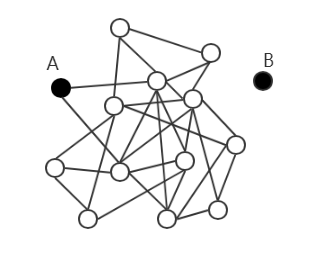
\includegraphics[width=0.6\linewidth]{Wwuxiangtu.png}
  \caption{节点度的示意图}
\end{figure}

在复杂网络中度为0的节点成为孤立节点.如图2-1所示是一个无向图,
节点A的度数为2,节点B为一个孤立节点.

一个节点最简单最重要的局部特征就是节点的度,网络中所有节点度的平均值称为网络的平均度,
用$<k>$来表示, 

\begin{equation}
<k>  = \frac{1}{N} \sum_{v \in V}^{}d(v).
\end{equation}

网络中节点度值分布特征是网络的重要几何性质,
度分布(Degree distribution)是表示网络中节点度分布状况的函数,一般用$P(k)$表示.

在规则网络中,各个节点具有相同度值$k_0$,网络第度分布服从$\delta$分布,即

\begin{equation}
  P(k) = \delta_0(k) = 
  \left\{
    \begin{array}{lr}
      1, & k = k_0,\\
      0, & k\neq k_0.
    \end{array}
  \right.
\end{equation}

在随机网络中,度分布服从泊松分布,主要特征是网络中大多数的节点的度值大致相同,
在平均度$<k>$处度分布有一个峰值,远离峰值的两边呈指数衰减,如下图2-2所示:
\begin{figure}[h!]
  \centering
  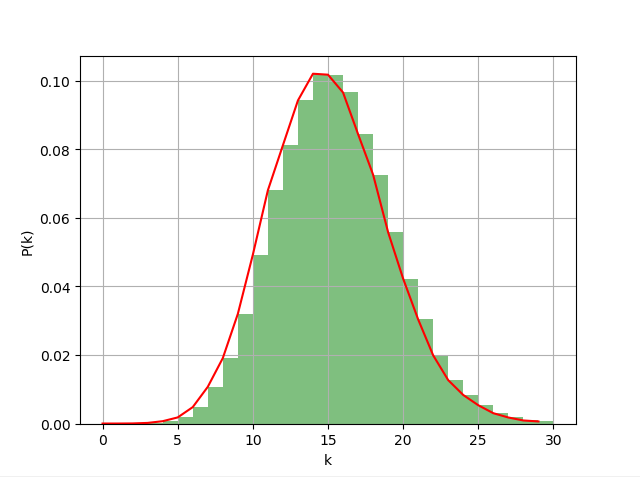
\includegraphics[width=0.6\linewidth]{Wposong.png}
  \caption{泊松分布}
\end{figure}

Albert等人研究了一个包含325739节点的万维网子网,
他们发现万维网的度分布不想规则网络和小世界网络那样是对称的泊松分布,
而是幂率分布(Power law distribution).
如图2-3所示为幂率分布函数图,从图中易知曲线没有峰值,且随k的增大而衰减.
从图中还可以知道大多数节点但仅有少量的连线,而少数节点拥有大量的连线,
具有大量连线的节点成为中枢点(Hubs),网络中节点具有很强的异质性.

\begin{figure}[h!]
  \centering
    \begin{subfigure}[b]{0.4\linewidth}
      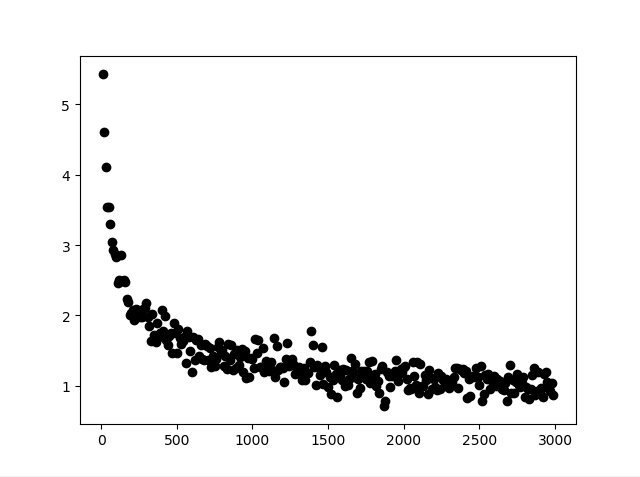
\includegraphics[width=\linewidth]{Wmilv.png}
      \caption{}
    \end{subfigure}
    \begin{subfigure}[b]{0.4\linewidth}
      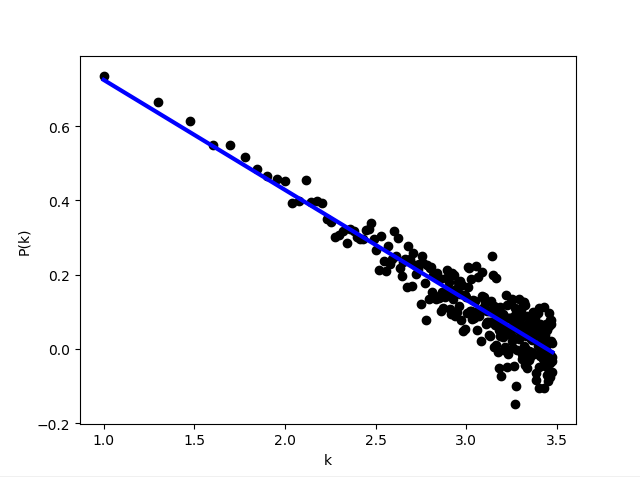
\includegraphics[width=\linewidth]{WmilvN.png}
      \caption{}
    \end{subfigure}
  \caption{幂律分布}
\end{figure}

网络度分布服从泊松分布还是幂律分布,反映了网络中节点之间是同质或异质的,
进而可以分析网络的很多性质.指数函数在半对数坐标系中是一台哦直线,
而幂律分布在双对数坐标系中是一条直线,因此为了区分度分布函数是指数衰减还是幂律衰减的,
我么只需要把度分布函数在半对数或双对数坐标系中划出其图像,通过观察即可区别开.


\subsection{聚类系数}
聚类系数(Clustering coeffocient)就是表示一个图形中节点聚集程度的系数,
实验结果证明显示,在现实世界的网络中,尤其在特定的网络中,
由于相对高密度连接点的关系,节点总是去向建立一组严密的组织.
在现实世界的网络,这种可能性往往比这两个节点但之间随机设立了一个连接的平均概率要大.
目前聚类系数的定义主要有以下两种:

\begin{definition}
  考虑到节点$v_i$的聚集系数,若其度数为$k_i(N)$,则在它的邻域(与节点$v_i)$
  有连线的节点全体)中,最多有$C_{k_i(N)}^{2} = \frac{k_i(N)(k_i(N)-1)}{2}$条线.
  如果他们的邻域中存在的连线数为$E(i)$,那么节点$v_i$的聚类系数定义为
  \begin{equation}
    C_i = \frac{E(i)}{C_{k_i(N)}^{2}} = \frac{2E(i)}{k_i(N)(k_i(N)-1)}
  \end{equation}
  其中,N表示网络中节点的总数.网络的聚类系数定义为网络中所有节点聚类系数的平均值,
  即
  \begin{equation}
    C = \frac{1}{N}\sum_{i = 1}^{N}C_i.
  \end{equation}
\end{definition}

Nollobas等人认为网络聚类系数采用加权平均值来代替式(2-4)更为合理,则网络聚类系数定义为:

\begin{equation}
  C = \sum_{i=1}^{N}C_i \frac{C_{k_i(N)}^{2}}{\sum_{j=1}^{N}C_{k_j(N)}^{2}}
    = \frac{\sum_{j=1}^{N}E(i)}{\sum_{j=1}^{N}C_{k_j(N)}^{2}}
\end{equation}

\begin{definition}
首先计算网络三个连通节点的总数,然后计算网络中三角形的总数,网络的聚类系数定义为:
  \begin{equation}
    C = \frac{3 \times \text{三角形的总数}}{\text{网络中三个连通节点的总数}}.
  \end{equation}
\end{definition}



\section{复杂网络模型}
\subsection{ER随机网络模型}
随机网络就是如果节点不按照确定的规则连接,而是以一定的概率连接,所得的网络.

20世纪60年代,匈牙利数学家Erdos和Renyi提出了ER随机网络模型.
对于ER随机网络模型有两种不同的生成机制.
(1)给定网络节点总数N,网络中任意两个节点以概率$p$连线,生成的网络全体记为$G(N,p)$,
构成一个概率空间.由于网络中连接数目是一个随机变量$X$,取值可以从0到$\frac{N(N-1)}{2}$,
有$n$条连线的网络数目为$C_{\frac{N(N-1)}{2}}^{n}$,
其中一个特定网络出现的概率为$P(G_n) = p^n(1-p)^{\frac{N(N-1)}{2} - n}$.
因此可生成不同的网络总数为$2^{\frac{N(N-1)}{2}}$,它服从二项分布.
网络中节点的平均连线数为$p\frac{N(N-1)}{2}$.



% \begin{figure}[h!]
%   \centering
%   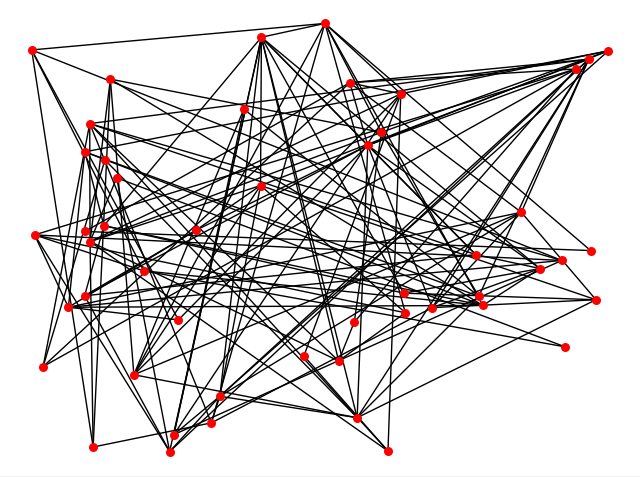
\includegraphics[width=0.6\linewidth]{WER-1.png}
%   \caption{具有50个节点,连接概率$p=0.1$的ER随机网络}
% \end{figure}

如图2-4(a)所示是一个具有50个节点,节点之间的连接概率为$p = 0.1$的ER随机网络.
网络中的节点平均度数为$<k> = 4.8$,网络的聚类系数为$C = 0.1068$.
如图2-4(b)所示是一个具有100个节点,节点之间的连接概率为$p = 0.0.05$的ER随机网络.
网络中的节点平均度数为$<k> = 4.98$,网络的聚类系数为$C = 0.03735$.

\begin{figure}[h!]
  \centering 
  \begin{subfigure}[b]{0.49\linewidth}
    \centering
    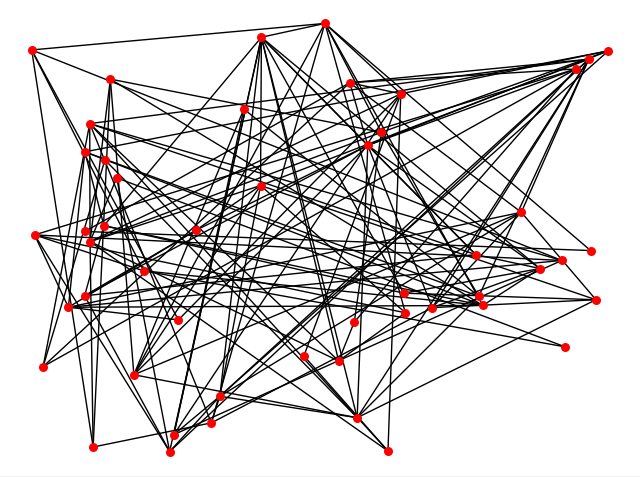
\includegraphics[width=\linewidth]{WER-1.png}
    \caption{N=50,p=0.1}
  \end{subfigure}
  \begin{subfigure}[b]{0.49\linewidth}
    \centering
    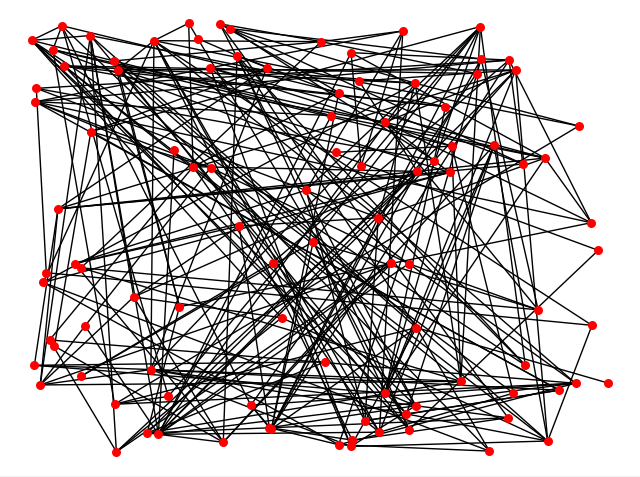
\includegraphics[width=\linewidth]{WER-2.png}
    \caption{N=100,p=0.05}
  \end{subfigure}
  \caption{第一种机制生成ER随机网络模型}
\end{figure}

% \begin{figure}[h!]
%   \centering
%   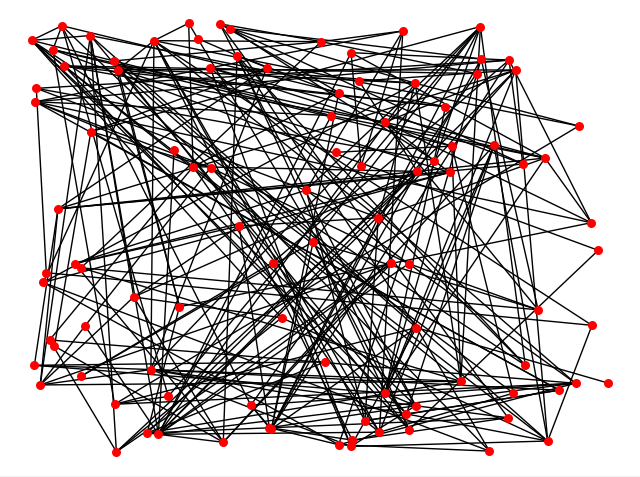
\includegraphics[width=0.6\linewidth]{WER-2.png}
%   \caption{具有100个节点,连接概率$p=0.0.05$的ER随机网络}
% \end{figure}


(2)给定网络节点总数N,随机连接网络中的n条边,
而这些连线是从总共$\frac{N(N-1)}{2}$条可能的连线中随机选取的,
生成网络全体记为$G(N,n)$,构成一个概率空间.这样生成的不同网络的总数为$C_{\frac{N(N-1)}{2}}^{n}$,
它们出现的概率相同,服从均匀分布,网络中两个节点连线的概率为$\frac{2n}{N(N-1)}$.

\begin{figure}[h!]
  \centering 
  \begin{subfigure}[b]{0.49\linewidth}
    \centering
    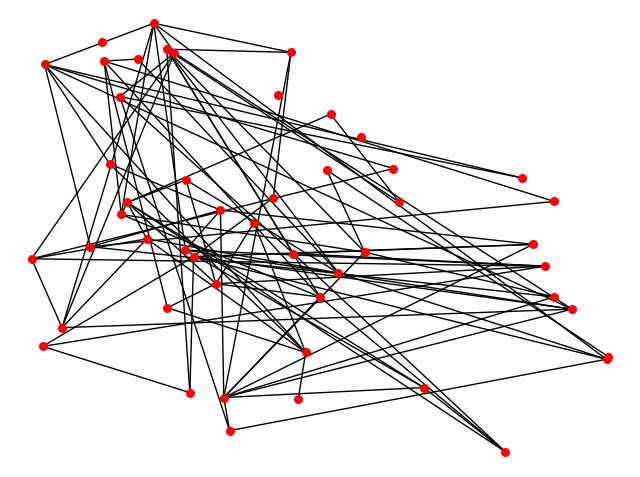
\includegraphics[width=\linewidth]{WER-3.png}
    \caption{N = 100,m = 100}
  \end{subfigure}
  \begin{subfigure}[b]{0.49\linewidth}
    \centering
    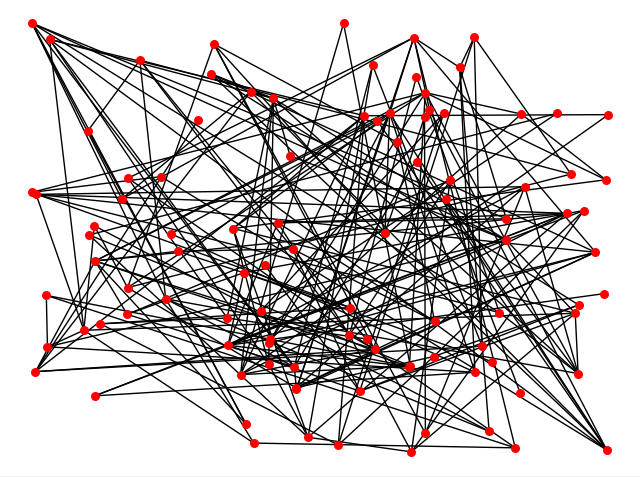
\includegraphics[width=\linewidth]{WER-4.png}
    \caption{N = 100,m = 200}
  \end{subfigure}
  \caption{第二种机制生成ER随机网络模型}
\end{figure}

% \end{figure}
% \begin{figure}[h!]
%   \centering
%   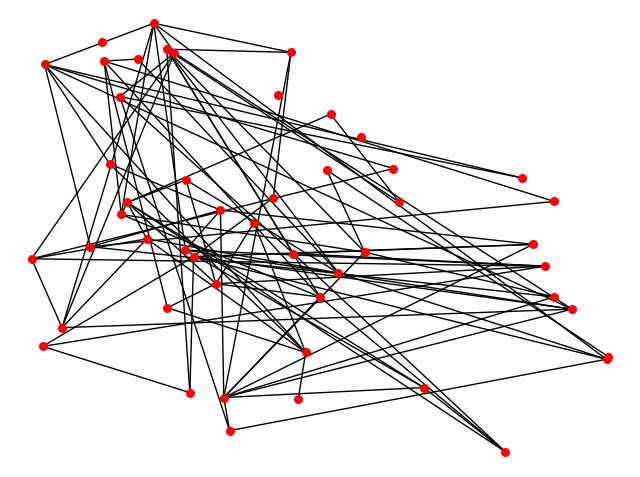
\includegraphics[width=0.6\linewidth]{WER-3.png}
%   \caption{具有100个节点,100条连线ER随机网络}
% \end{figure}

如图2-5(a)所示是一个具有50个节点,100条连线的ER随机网络.
网络中的节点平均度数为$<k> = 3.96$,网络的聚类系数为$C = 0.08092$.
如图2-5(b)所示是一个具有100个节点,200条连线的ER随机网络.
网络中的节点平均度数为$<k> = 4.06$,网络的聚类系数为$C = 0.07368$.

% \begin{figure}[h!]
%   \centering
%   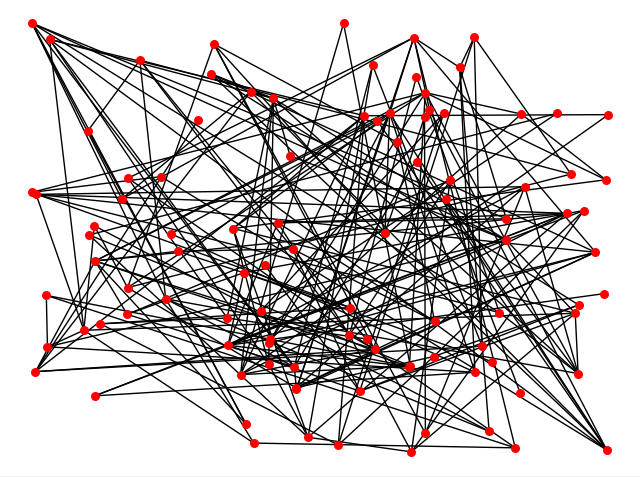
\includegraphics[width=0.6\linewidth]{WER-4.png}
%   \caption{具有100个节点,200条连线ER随机网络}
% \end{figure}

对于ER随机网络的两种生成机制,
当$p\frac{N(N-1)}{2} = n$时,模型$G(N,p)$和$F(N,n)$是等价的.
当网络中的节点数N比较大时,ER随机网络的节点度分布可以近似为泊松分布,
由于网络中存在大量的随机连线,网络的聚类系数比较小.

\subsection{WS小世界网络模型}
通过研究发现,规则网络具有比较大的聚类系数,
但随着网络规模的增大,它的平均路径长度也很大;
而对于随机网络,虽然它有较小的平均路径长度,但其聚类系数也很小.
为了更好的发现实际网络的内在机制,Watts和Strogatz在1998年提出了小世界模型.
WS小世界网络模型的生成机制如下:

(1)初始:给定一个具有N个节点的环,
环上每个节点都与它最邻近的K=2k个节点但相连,构成一个最近邻环网络.

(2)重连:以概率p对环网中的每条连线进行重新连线,方法是将选择的每条连线的一端断开,
然后随机的连接到其他的节点桑,不允许自连线和重复连线.

通过最近网络随机重连得到的WS小世界网络模型的很多性质介于规则网络和随机网络之间,
通过调节重连概率p可以实现从规则网络p=1到随机网络p=1的过度.
由于在规则网络中进行重连,使得网络中存在随机的连线,形成捷径,
从而网络中节点间的最短路径长度大大减少.
由此我们可以看出WS小世界网络模型具有较小的平均路径长度和较大的聚类系数.

\begin{figure}[h!]
  \centering
  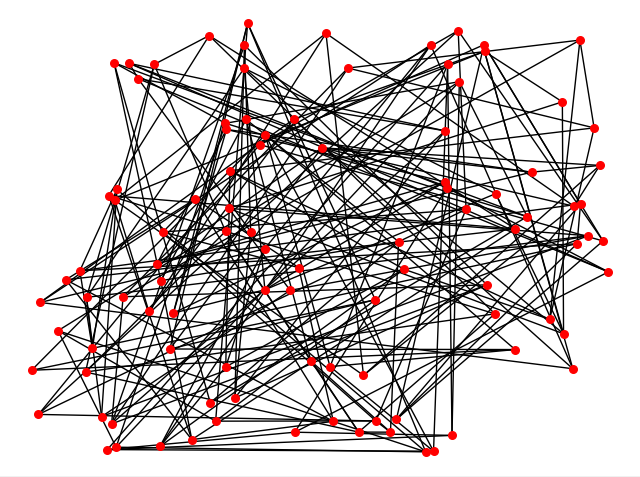
\includegraphics[width=0.6\linewidth]{WWS.png}
  \caption{WS小世界网络模型(N=100,K =4,p=0.04)}
\end{figure}

如图2-6所示是一个具有100节点,每个节点与最近邻的4个邻居相连,重连概率为0.04的WS小世界网络模型.
网络中节点的平均度$<k> = 4$,网络的聚类系数$C = 0.4127$.


\subsection{BA无标度网络模型}
1999年,Barabasi和Albert在研究万维网时发现,万维网的度分布不想随机网络和小世界
那样具有对称的泊松分布,而是便宜的幂率分布.在该网络中,大多数节点仅有少量连线,
而少数节点拥有大量的连线.为此他们提出了无标度(scale-free)网络模型,
揭示了增长和择优机制在复杂网络自组织演化过程中的普遍性和幂律的重要性.
BA无标度网络模型的生成机制如下:

(1)初始:开始时给定一个含有$n_0$节点以一定的规则连接的网络;

(2)增长:在每个时间步增加一个带有$m(m \leq n_0)$条信赖年界限的新节点;

(3)择优:新节点以择优概率

\begin{equation}
  \prod (k_i) = \frac{k_i}{\sum_{j}^{}},
\end{equation}
选择旧节点i与之连线,其中$k_i$世界点i的度数.

这个模型提出了两条重要的网络演化机制:增长和择优,这是从万维网实际形成过程中抽象出来的,
万维网每时每刻都有新的网页增加.增长和择优是生成无标度网络不可缺少的内在机制.
无标度网络中的节点具有异质性,不同度的节点在网络中的重要程度不同.
在社会网络中,都可以表示个体的作用力和影响都,一个点的度越大,
一般表示在整个网络系统组织中的作用和影响越大,反之亦然.

\begin{figure}[h!]
  \centering 
  \begin{subfigure}[b]{0.49\linewidth}
    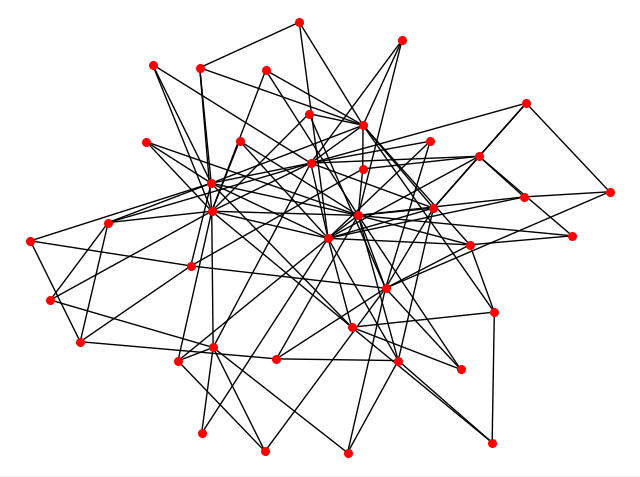
\includegraphics[width=\linewidth]{WBA-1.png}
    \caption{N=40,m=3}
  \end{subfigure}
  \begin{subfigure}[b]{0.49\linewidth}
    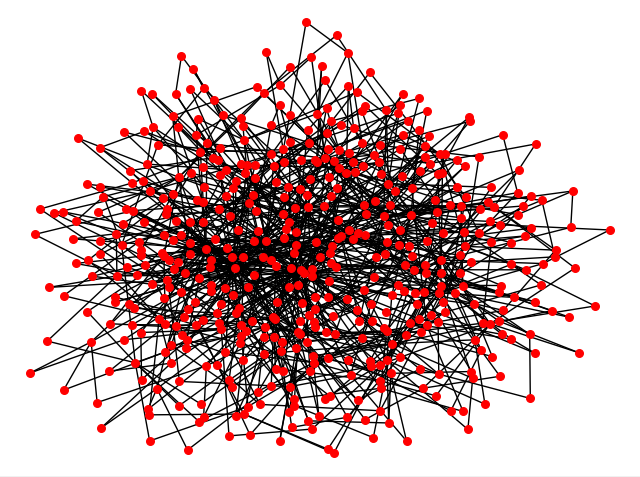
\includegraphics[width=\linewidth]{WBA-2.png}
    \caption{N=500,m=2}
  \end{subfigure}
  \caption{BA无标度网络模型}
\end{figure}

如图2-7(a)所示是一个具有40个节点,每个节点新加入的节点带有3条新连接线的BA无标度网络模型.
网络中的节点平均度数为$<k> = 5.55$,网络的聚类系数为$C = 0.2993$.
如图2-7(b)所示是一个具有500个节点,每个节点新加入的节点带有2条新连接线的BA无标度网络模型.
网络中的节点平均度数为$<k> = 3.984$,网络的聚类系数为$C = 0.03618$.

BA无标度网络模型的度分布严格服从指数为3的幂率分布,
当网络规模较大时,网络具有较小的平均路径长度,但是网络的聚类系数也比较小.
BA无标度网络模型可以魔术一大类实际的网络,揭示了增长和择优时长生无标度的内在机制.


\subsection{其他网络模型}

当然除了本章节所介绍的三种网络模型以外,还有其他模型,
比如Bollobas提出的LCD(Linearized chord diagrams)模型、
Liu等人提出的混合连接网络模型以及Zhang等人提出的广义的合作网络(两者都属于具有随机和则有连线规则的网络模型)、
Holme和Kim提出的HK网络模型都能够描述一大类网络特性,本文就不再继续介绍相关知识,有兴趣的可以查阅资料了解.

\section{复杂网络度分布的求解方法}
\subsection{平均场方法}
Barabasi等人为了分析BA模型的度提出了平均场方法(mean-field approach).
具体步骤如下:
% 令$k_i(t)$表示节点$i$(在第i时刻加入到网络的节点)在时刻t的度数,
对于BA模型,
% 在t时刻网络共增加了m条线,每条线连接网络中的两个节点,
% 此时网络中节点的读书之和$\sum_{i}^{}k_i(t)\approx 2mt$.
根据连续性理论,把$k_i(t)$看作连续动力学函数,则$k_i(t)$满足如下的动力学方程:

\begin{equation}
  \frac{\partial k_i(t)}{\partial t} = 
  m\prod (k_i(t)) = \frac{k_i(t)}{2t}
\end{equation}

$$k_i(t) = m.$$
上述方程有如下解:
\begin{equation}
  k_i(t) = m\left( \frac{t}{t} \right)^{1/2}.
\end{equation}
由于节点是随机选择的,因此$i$在所有节点中服从均匀分布,
又初始网络中含有$n_0$个节点,从而$\rho (i) = \frac{1}{t+n_0}$.由式(2-10),可得

\begin{equation}
  P\{k_i(t)<k\} = P\left\{ i>\frac{m^2t}{k^2}\right\}
  = 1-\frac{m^2}{k^2(t+m_0)},
\end{equation}
对$k$求导即可得到$P(k,t)$:
% ($P(k,t)$表示在时刻t的度数为k的节点所占比例)

\begin{equation}
  P\{k_i(t)<k\} = \frac{\partial P\{k_i(t)<k\}}{\partial k} = 
  2m^2k^{-3}\frac{t}{t+n_0}
\end{equation}
当$t \rightarrow \infty$时,网络稳态分布为:

\begin{equation}
  P\{k\} = \lim_{t \rightarrow \infty} P\{k_i(t)<k\} \propto 2m^2k^{-\lambda}
\end{equation}
其中,$\lambda =3$为标度指数,$k_i(t)$表示节点$i$在时刻t的度数,$m$表示在$t$时刻增加的连线.

通过平均场方法得出BA模型的度分布服从指数为3的幂律分布.

\subsection{率方程方法}
Krapivsky等人在分析网络度分布时提出了率方程方法(rate-equation approach),
率方程方法的求解如下:
% 令$N_k(t)$在t时刻网络中的度数为$k$的节点的总数,
对于BA模型,
% $\sum_{k}^{}kN_k(t)\approx 2mt.$
根据连续性理论,现在考虑节点数的变化率,
% 对于原来度数为$k-1$的节点由于与新节点但相连度数变为$k$,需要算入,
% 对于原来度数为$k$的节点,由于增加了连线度数变为$k+1$,需要排除;对于新节点,
% 它的度数恰好为$m$,若$k=m$,则需要保留.
节点与新加入的节点相连的概率为
$m \frac{k_i(t)}{\sum_{k}^{}N_k(t)}$,
可得到关于$N_k(t)$的率方程:
\begin{equation}
 \frac{dN_k(t)}{dt} = N_{k-1}(t)\frac{k-1}{\sum_{k'}^{}k'N_{k'}(t)} - N_k(t)m
 \frac{k}{\sum_{k'}^{}k'N_{k'}(t)} + \delta_{k,m}.
\end{equation}
由大数定律得
$$\lim_{t \rightarrow \infty}E\left( \frac{N_k(t)}{t}\right) = P(k)$$
式(2-12),可表示为
\begin{equation}
  (k+2)P(k) = (k-1)P(k-1) + 2\delta_{k,m}.
 \end{equation}
 式(2-13)是一个关于P(k)的一阶差分方程,解此差分方程可得:
 \begin{equation}
  P(k) = \frac{2m(m+1)}{k(k+1)(k+2)} \propto 2m^2k^{-3}.
 \end{equation}
其中$N_k(t)$表示在t时刻网络中的度数为$k$的节点的总数

 通过率路方法得到的BA模型的度分布服从3的幂律分布,此结果与用平均场方法所得结果一致.

\subsection{其他方法}
Bollobas等人用靶方法严格证明了LCD模型度分布的存在行并求出了度的表达式:

\begin{equation}
  \lim_{t \rightarrow \infty}P(k,t) = P(k).
\end{equation}

侯振挺等人在BA模型应用马氏链理论的首达概率及其方法和技巧,
给出了网络度分布的精确表达式如下:

\begin{equation}
  P(k) = \frac{2m(m+1)}{k(k+1)(k+2)}
  \propto2m(m+1)k^-3
\end{equation}

马氏链方法在求解复杂网络度分布中,具有一定的普适性,
他们对增长网络和演化网络的度分布进行了系统的分析,
对增长网络、混合网络和演化网络的度分布问题给出一个统一的解答.

这些方法就不再给出详细的证明过程,只给出一些结论。有兴趣的可以查阅资料了解相关内容.






\chapter{}
本章节详细介绍提出的融合句法结构的深度神经网络模型(下文简称:融合模型).
该模型是将蕴含语言学知识的依存句法结构信息融合到传统的LSTM模型中,
以提升文本理解的效果.
\section{模型设计}
这个部分将说明如何对文本内容和语言学知识进行向量化的编码,
并着重说明融合模型的架构,详细说明各个模块的运作方式.
\subsection{词向量设计}
有两个词向量的设计工作,第一是将文本的向量化,第二是将依存句法结构向量化.

对于第一个文本的向量化,可以采用先前介绍的Glove模型来训练词向量,
或者直接从官网https://nlp.stanford.edu/projects/glove/上下载已经训练好的词向量.
这些词向量是通过英文维基百科训练的,维度有多种,包括50,100,200,300维等.
设每个单词表示成一个$d$维的向量$e_{i}^{w} \in \mathbb{R}$,所以一段文本可以表示为
$E^{w} \in \mathbb{R}^{d \times N_{w}}$,其中$N_{w}$表示这段文本的长度.

对于第二个依存句法结构的向量化,首先通过斯坦福句法分析工具包生成依存句法树.
这样可以获得依存句法树根节点到叶子节点的形成的子结构.

比如,对于句子“show me the flights from seattle to san francisco.”
可以获得的子结构如下图所示.

\begin{figure}[h!]
  \centering
  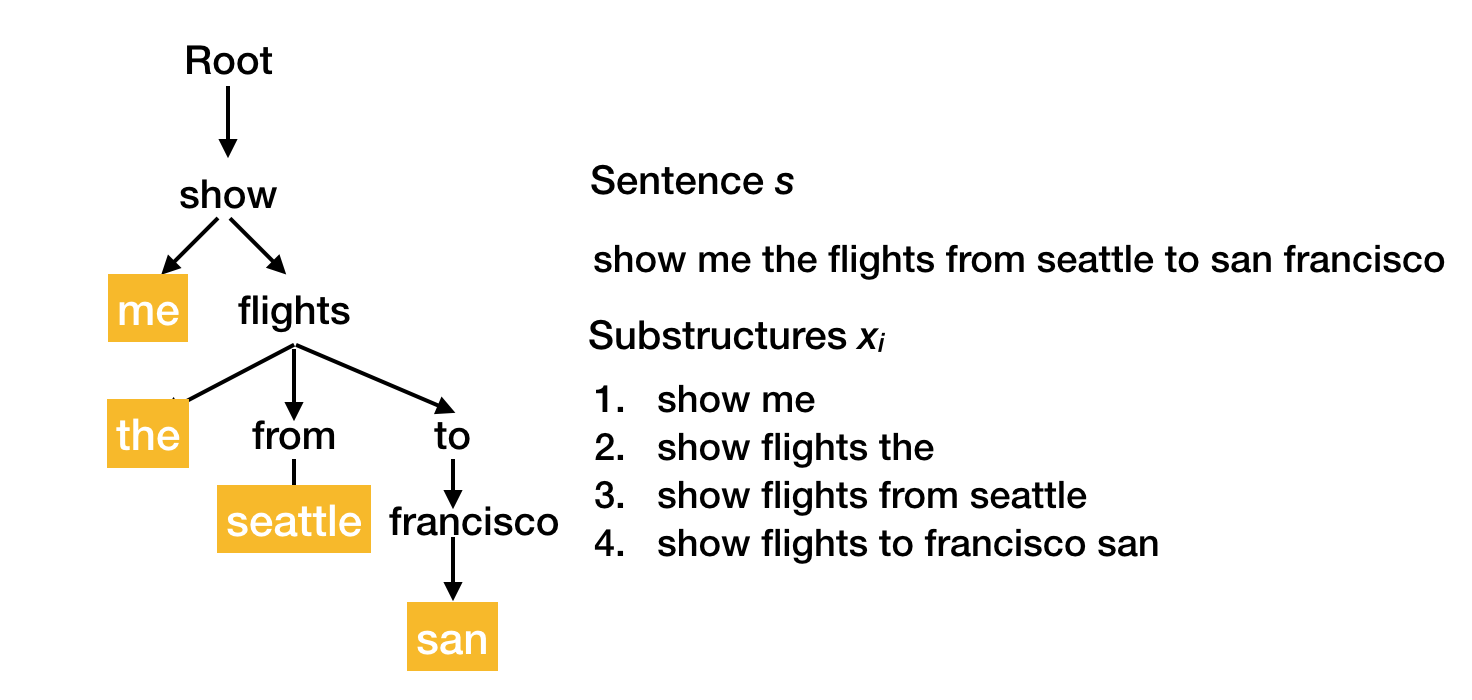
\includegraphics[width=0.8\linewidth]{yicunjufashujuli.png}
  \caption{根据依存句法树获得子结构}
\end{figure}

这样上面图中的依存句法结构就可以通过这4个子串$x_{1},x_{2},x_{3},x_{4}$来表示,
事实上仅仅通过这4个子串就可以反过来推导出依存句法树,
所以依存句法树和其从根节点到叶子节点的子串是相互唯一确定的.

下面对这4个子串进行向量化,每个单词依然表示成一个$d$维的向量,
那么一个子串$x_{i}$就可以表示为$E_{x_{i}} \in \mathbb{R}^{d*N_{x_{i}}}$,
这里$N_{x_{i}}$表示子串$x_{i}$的单词个数.
值得注意的是所有子串的总数一定是小于文本中所有单词数量的,
因为子串是根据叶子节点获得的,非叶子节点就没有对应的子串,
这样也可以减少模型中的重复信息.

最后还需要说明一下,如何根据依存句法树中获得所有从根节点到叶子结点的子串,
事实上可以通过一个简单的递归算法解决,具体如下.

\begin{table}[h!]
  \centering
  \begin{tabular}{l}
    \toprule
    \textbf{递归获取依存句法树子串算法描述} \\
    \midrule
    (1)输入: 依存句法树Tree \\
    (2) 定义所有子串的列表$all\_substructures$,路径字符串$path$ \\
    (3) 定义递归函数$walk(node,path)$,$node$为当前节点 \\
    (3.1) 路径字符串加上当前节点的值 $path = path + node.value$ \\
    (3.2) 判断当前节点是不是叶子结点,如果是转到(3.3),如果不是转到(3.4)\\
    (3.3) 所有子串的列表加上当前的路径字符串,$all\_substructures.append(path)$ \\
    (3.4) 对该节点所有的子节点递归调用,$walk(node.childnode,path)$ \\
    (4)调用 $walk(Tree.root\_node,path)$ \\
    (5)输出所有子串的列表$all\_substructures$ \\
    \bottomrule
  \end{tabular}
  \caption{递归获取依存句法树子串算法描述}
\end{table}
通过上面的算法输入依存句法树就可以获取所有的子结构.

\subsection{模型架构}
融合句法结构的深度神经网络模型的整体架构如下图所示:
\begin{figure}[h!]
  \centering
  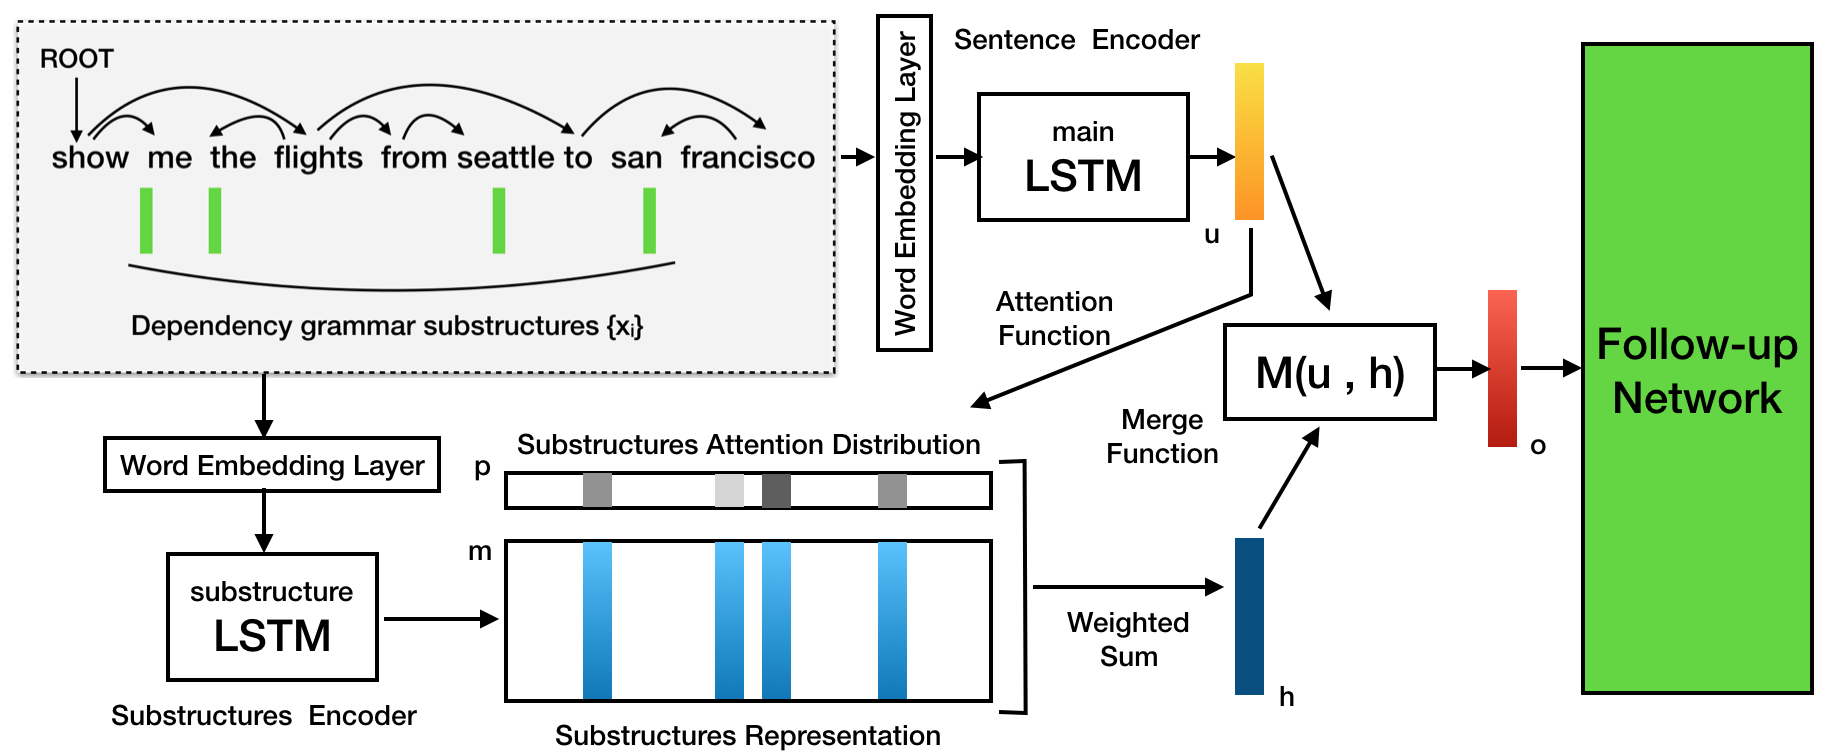
\includegraphics[width=0.95\linewidth]{model.png}
  \caption{融合句法结构的深度神经网络模型}
\end{figure}

整个模型图示从左向右看子结构句子和主文本句子分别通过两个LSTM模型,
将子结构输出的结果加权平均后与主文本句子的输出结果相融合,
得到一个最终的融合表示,最后将这个表示送入后续的神经网络中,
完成文本分类、机器翻译等文本理解的应用.下面对具体的阐述模型中的几个细节.

(1) 这里的词嵌入层直接采用Glove的词向量,只需要将单词与词向量进行一一映射即可.
词向量的维度$d$是模型的超参数.

(2)LSTM模块采用单层经典的LSTM模型即可,事实上在本模型中,LSTM可以看成一个编码器,
我们只取LSTM的最后一个隐藏层节点,因为LSTM具有记忆的功能,
所以最后一个节点可以认为是对整个输入文本的编码.
所以$x_{i}$被编码成$m_{i}$,整个文本句子$s$被编码成$u$,
其中$m_{i} \in \mathbb{R}^{H_{sub}}$ ,$H_{sub}$为子结构LSTM隐藏层节点个数,
$u \in \mathbb{R}^{H_{main}}$,$H_{main}$为主LSTM隐藏层节点个数.

\begin{equation}
\left\{
  \begin{array}{l}
   m_{i} = LSTM_{sub}(x_{i}) \\ 
   u = LSTM_{main}(s) \\ 
  \end{array}
  \right.
\end{equation}

LSTM的内部推倒可以见2.2.2小节,
下面通过一个图示来说明通过LSTM模型的过程,
一个子结构句子“show me the”通过LSTM,
并将最后一个隐藏层输出作为编码结果$m$.

\begin{figure}[h!]
  \centering
  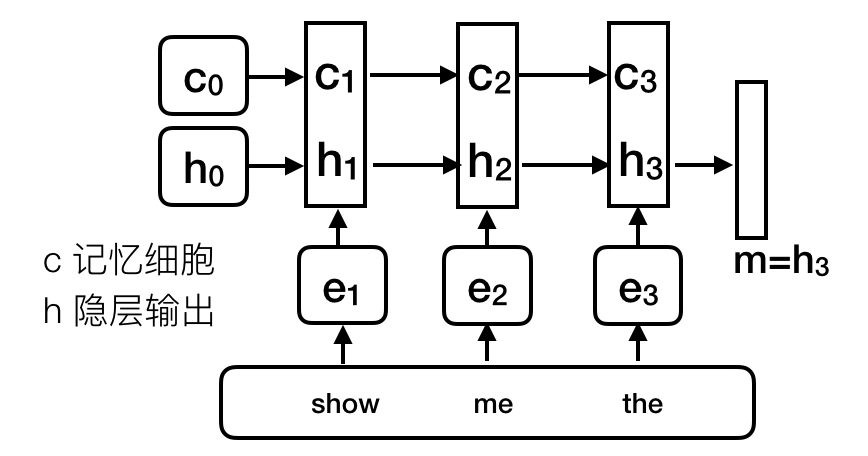
\includegraphics[width=0.5\linewidth]{LSTMjuti.png}
  \caption{$x$通过LSTM编码得到$m$}
\end{figure}

(3)
通过Attention函数来计算整个句子的编码$u$和每一个子结构$m_{i}$的匹配程度.

具体可以分成两步,打分函数$Socre\_Function$和$softmax$函数,
首先通过打分函数计算相关性的评分,然后再通过sotfmax来计算匹配概率$p_{i}$,
这里的$p_{i}$就可以认为是每一个子结构对
理解这个文本的重要程度.

\begin{equation}
  \left\{
    \begin{array}{l}
     socore_{m_{i}} = Socre\_Function(u,m_{i}) \\ 
     p_{i} = softmax(socore_{m_{i}}) \\ 
     softmax(z_{i}) = \frac{e^{z_{i}}}{\sum_{j} e^{z_{j}}}
    \end{array}
  \right.
\end{equation}

这里的打分函数有多种表达形式,具体会在下一节中着重说明.

(4)
$h$是子结构加权平均的结构,可以用来表现句子依存句法结构的信息,
也就是说这个向量事实上代表了文本$s$的语言学知识.

\begin{equation}
  h = \sum_{i}(p_{i}m_{i})
\end{equation}

(5)
向量$o$是主文本LSTM输出$u$和文本子结构LSTM输出加权$h$融合的结果.
可以作为整个融合模型的输出,送入到后续的网络中.
\begin{equation}
  o = M(u,h)
\end{equation}

式子中的函数$M$是融合函数,有多种融合方式,具体会在后面的小节中着重说明.

(6)后续的网络,事实上可以接入任何形式的网络,完成众多不同的文本理解任务.
因为这个融合模型的初衷就是可以无缝替换原先的LSTM模型,所以融合模型的输入和输出,
与传统的LSTM模型的输入和输出是完全相同的,
不过融合模型的输出中附加了句法结构的语言学知识.

如后续网络接入情感分类(简化仅有两类情感)网络,如下图所示.
把融合网络的输出向量$o$,
接到一个全连接的神经网络中,网络为了简化,这里只有一层,也就是两个隐藏层节点,
后面再接一个softmax层,就可以获得这个文本两类情感的概率分别是多少,
取概率较高的类别作为最终的情感类别.
\begin{figure}[h!]
  \centering
  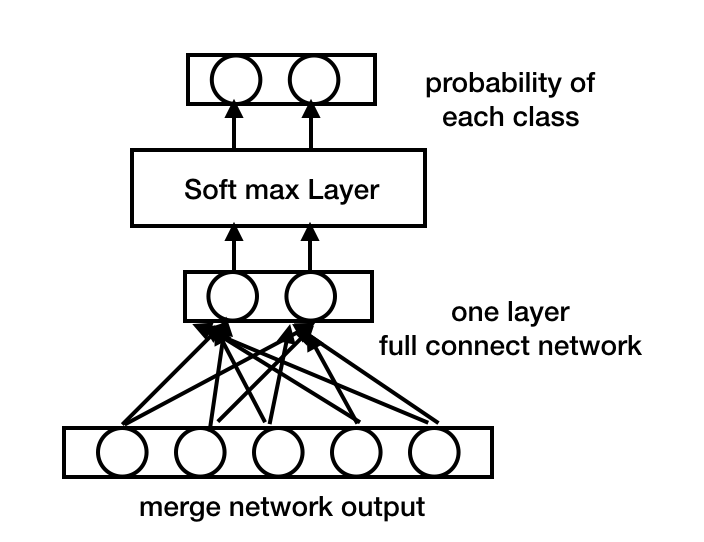
\includegraphics[width=0.5\linewidth]{erfenlei.png}
  \caption{后续接入情感分类网络}
\end{figure}

再如后续网络接入1toM网络,就可以实现一个机器翻译的网络,如下图所示.
把融合网络的输出向量$o$,接到到LSTM中,这样每个隐层的输出$y_{i}$,
就构成了一个序列的向量,进而把每个$y_{i}$映射成字符$w_{k}$,
这样取得了一连串的字符输出,可以作为一个简化的机器翻译网络.

\begin{figure}[h!]
  \centering
  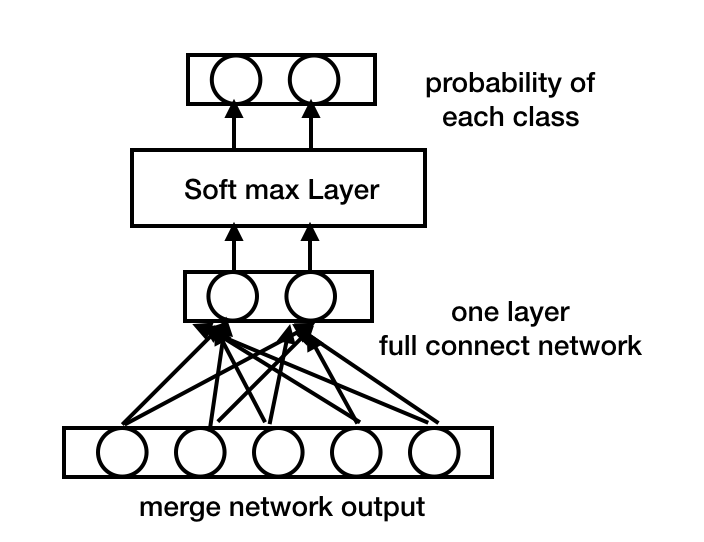
\includegraphics[width=0.5\linewidth]{erfenlei.png}
  \caption{后续接入LSTM网络}
\end{figure}

所以将融合模型的输出$o$,结合先2.2.1小节提到的1 to 1 、1 to N模型,
就可以实现众多的文本理解任务. 

\section{句法结构Attention机制}
句法结构的Attention机制是为了计算出哪个子结构对文本的理解更重要.
所以通过引入Attention机制,可以让网络学习出文本中对整个文本内容相对核心的子结构.
如上一节所说,主要是讨论如何构建打分函数,
得到了当前子结构$m_{i}$,$m_{i} \in \mathbb{R}^{H_{sub}}$与源文本$u$,$u \in \mathbb{R}^{H_{main}}$相关度的评分,
然后采用softmax公式将相关度转换成概率,由此完成了整个Attention机制.
常见的Attention模型包括:dot Attention、bi-liner Attention和concatention-based Attention.

(1)dot Attention

这种Attention机制最为简单,首先需要
构造一个维度平衡矩阵$W$,$W \in \mathbb{R}^{H_{main} \times H_{sub}}$,
所以打分函数可以表示为:

\begin{equation}
  score_{m_{i}} = u^{T}Wm_{i}
\end{equation}

一般采用dot Attention的场合,特别的会$H_{main} = H_{sub}$,这样就只需要点乘即可.

\begin{equation}
  score_{m_{i}} = u^{T}m_{i}
\end{equation}

(2)bi-liner Attention

这个Attention是在dot Attention的基础上构造一个矩阵$W$,$W \in \mathbb{R}^{d \times d}$连续乘其本身和它的转置.
同样一般会有$H_{main} = H_{sub} = d $.

\begin{equation}
  score_{m_{i}} = u^{T}WW^{T}m_{i}
\end{equation}


(3)concatention-based Attention

这个Attention相对比较复杂.
需要构造两个个维度平衡矩阵$W_{1}$,$W_{2}$,
其中$W_{1} \in \mathbb{R}^{d \times H_{sub}}$,
$W_{2} \in \mathbb{R}^{d \times H_{main}}$,
一个偏置向量$b$,$b \in \mathbb{R}^{d}$,
最后还需要一个维度平衡向量$v$,$v \in \mathbb{R}^{d}$.
整个打分函数可以表示如下:

\begin{equation}
  score_{m_{i}} = v^{T}activation(W_{1}m_{i}+W_{2}u+b)
\end{equation}

这里的激活函数一般选择ReLU,tanh即可.



\section{模型融合方式}
这里的融合就是将主文本LSTM的输出的向量$u$,$u \in \mathbb{R}^{H_{main}}$
与表现文本的句法结构的向量$h$,$u \in \mathbb{R}^{H_{sub}}$融合,
为了简化操作,这里假设$u$与$h$的维度是相同的,即$H_{main} = H_{sub}$.
事实上如果不相同,也只需要对于任意一个向量左乘一个平衡矩阵即可.
常见的融合方式,主要有相加融合和连接融合.

(1)相加融合

相加融合,顾名思义就是将$u$和$h$相加.

\begin{equation}
  o = u + h
\end{equation}

当然,这里也可以是有权重的相加,权重表现重要程度的不同.设权重系数为$\alpha$.
这里的$\alpha \in (0,1)$.

\begin{equation}
  o = \alpha u + (1-\alpha)h
\end{equation}

经验上,$\alpha$和模型效果的关系总体上服从先增加后减少的趋势,
所以通过实验可以搜索到对于某个特定任务上最佳的值.

(2)连接融合
连接融合,又可称为串联融合,是把两个向量直接在空间上串行拼接成一个新的向量,
这样新的向量的维度就是原先的两倍,所以需要在通过压缩矩阵$W$,$W \in \mathbb{R}^{d \times 2d}$,
把新的向量压缩成原来的维度.值得注意的是,这里的参数的$W$,也是一个需要学习的变量,不是模型设计初期就固定的.
融合方式具体如下图所示:
\begin{figure}[h!]
  \centering
  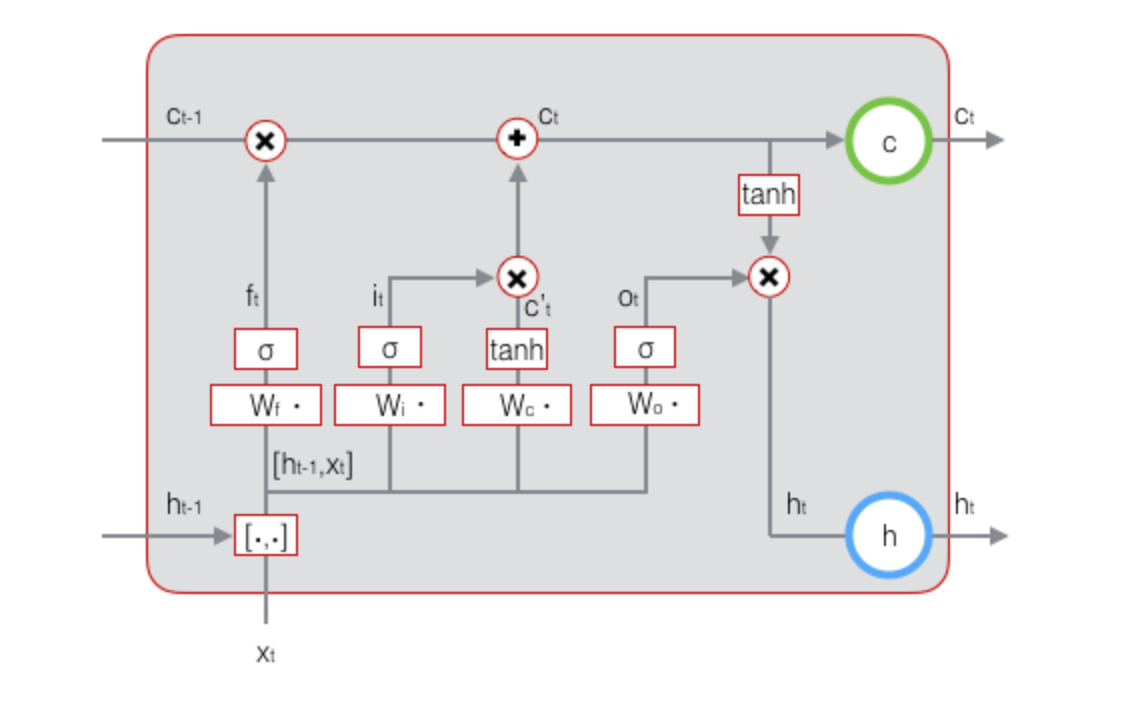
\includegraphics[width=0.4\linewidth]{LSTM.png}
  \caption{连接融合}
\end{figure}

对应到本模型上,连接融合就是是将两个向量串联,即$[u,h]$,最后再左乘$W$,
将其映射为原先的维度,公式如下:

\begin{equation}
  o = W[u,h]
\end{equation}

相加融合和连接融合是目前广泛应用的两种融合方式,在实践上
简单易行而且也能获得比较好的融合效果.
通过融合就能获得文本语义和文本结构的融合表示$o$,进而送入后续的网络中以完成不同的应用.


\chapter{聚类算法分析}
大数据不仅引起学术界和产业界的普遍重视,更上升为世界各国的国家战略.
然而,要充分发挥大数据的作用,必须具备强大的数据分析能力.
本章就无监督学习中的$K-means$算法进行研究,并分析算法的优缺点.
并将本章研究的算法运用到下一章节对具体数据进行聚类分析.

\section{聚类算法}
\subsection{简介}
什么是聚类呢?《周易·系辞上》说:“方以类聚,物以群分,吉凶生矣.”
聚类是把一个数据对象的集合划分成簇(子集),使簇内对象批次相似,
簇间对象不相似的过程,是大数据分析的基本工具.

机器学习包括监督学习和无监督学习.
监督学习的主要任务是分类,即用大量已标记数据完成对新数据的区别;
无监督学习的主要任务是聚类,即在没有任何人工干预情况下对数据进行区分.
无监督学习是大数据分析最基本的工具,
我们必须清楚的看到无监督学习难度远大于监督学习.


\subsection{聚类算法分类}
和分类(监督学习的主要任务)不同,
聚类是在无标记样本的条件下将数据分组,
从而发现数据的天然结构.聚类在数据分析中扮演重要的校色,
它通常被用于以下三个方面:

(1)	发现数据的潜在结构:深入洞察数据、产生假设、检测异常、确定主要特征.

(2)	对数据进行自然分组:确定不同组织之间的相似程度(系统关系).

(3)	对数据进行压缩:将聚类原型作为组织和概括数据的方法.

这几个方面的功能是聚类既可以作为预处理程序,又可以作为独立的数据分析工具.

通过查阅文件和上网查找资料,总结了聚类的发展阶段如下图所示:

\begin{figure}[h!]
  \centering
    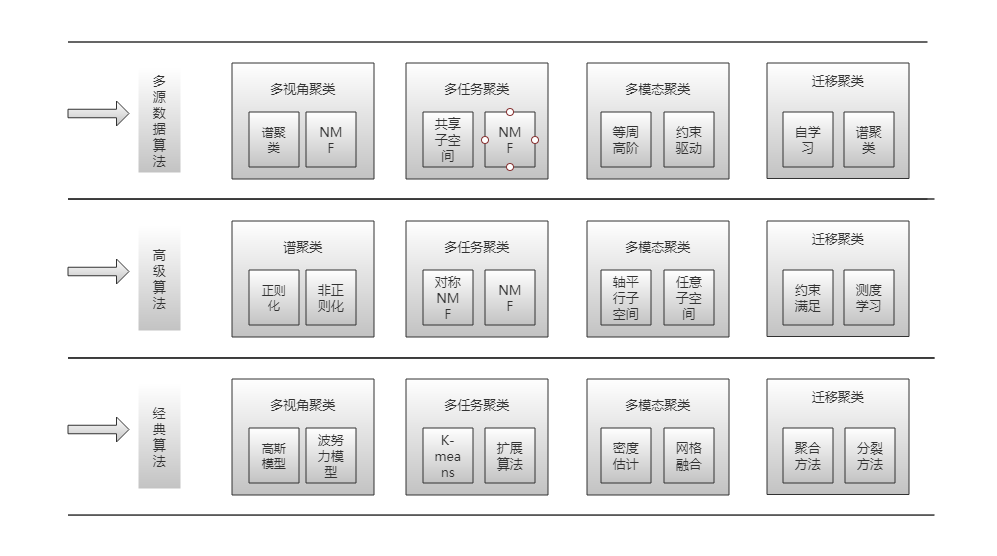
\includegraphics[width=1.0\linewidth]{Wjuleifazhan.png}
  \caption{聚类发展}
\end{figure}


\section{$K-means$算法}
\subsection{算法简介}
$K-means$算法是由Steinhaus与1955年、
Lloyd于1957年、Ball和Hall于1965年、
Mcqueen于1967年分别在各自的不同的科学研究领域独立提出来的.
自被提出来以来,这一算法在许多学科领域得到了大量的研究和应用,
具体的例如数据压缩、数据分类、密度估计等诸多方面.
由于其算法思想简洁易懂,
而且对于许多聚类问题都可花费较小的计算代价而得到不错的聚类结果,
$K-means$算法成为各种聚类算法中较为常用的算法之一,
至今仍然被广泛的使用,被学者们选为数据挖掘领域的十大算法之一.

\subsection{算法思想}
$K-means$算法继承了基于划分的聚类方法的基本思想.
基于划分的算法按某种目标将数据集划分成若干个组,
划分的结果就是使目标函数值最大化(或者最小化).
这样的优化目标通常是NP难的,因此采用某种贪心策略迭代求解.
具体的做法就是每个簇指定一个或者若干个代表点,
根据目标函数用这些代表点对这个数据集进行划分,
在划分结果中重新选择代表点,重复上述过程知道收敛.
贪心算法通常获得目标函数的局部最优解.
基于划分的算法基本上都以点对时间的聚类为标准,
而距离和簇代表点的选择至关重要.

$K-means$算法在如何产生一个划分方面,
$K-means$算法设定了每个划分的中心点,
从而形成以中心为分类依据的球星簇;
在验证所产生的划分是否合理方面,
$K-means$算法以划分的类内紧致性作为标准,
具体来说,是以点与点之间的距离之和作为度量准则.
这种划分标准以及度量标准保证了算法可以很快达到收敛,
这就是$K-means$算法相比于其他算法的一个重大优势.

\subsection{目标函数}
在K-menas算法中,
涉及计算每个对象与各个簇中心点之间的距离,
这个距离的度量也是用户自行设定的.
通常有闵可夫斯基、曼哈顿距离(L1范式)和欧几里得距离(L2)范式等.
针对不同的数据类型可以选取不同的距离度量标准.
在一般情况下,欧几里得是一个很好的度量数据间相似的标准,
也是大部分$K-means$算法中选定的距离度量标准.

聚类算法的目标通常用一个目标函数来表示.
采用欧几里得距离度量相似性的$K-means$算法,
使用误差的平方和(sum of squared errors,SSE)作为度量聚类质量的目标函数.
给定一个包含 $n$ 个数据对象的数据集合$D =\{ x_1, x_2, \cdots, x_n \}$,
定义经由$K-means$算法进行聚类分析后的产生的类别集合为$C=\{ C_1, C_2, \cdots, C_k \}$.
算法目标定义如下:
\begin{equation}
  \centering
  SSE(C) = \sum_{ k=1}^{n} \sum_{x_i \in C_k} {\parallel x_i - c_k \parallel}^2 \qquad 
\end{equation}
式中,$c_k$是簇$C_k$的中心点,计算方法如下所示:

\begin{equation}
  \centering
  c_k = \frac {{\sum_{x_i \in C_k}^{n}} x_i} {\mid C_k \mid} \qquad
\end{equation}

$K-means$算法的目标就是能找到能最小化$SSE$的聚类结果,
这个最优化问题是一个NP难问题,
难以找到一个多项式算法对其求解.
不过可以将此问题进行转化,
通过不断迭代更新簇的构成和簇的中心点来进行最优化的求解,
Lloyd算法就是此类算法.算法的迭代过程主要是:
第一步分配过程,在分配过程中,
每个数据样本都要被分配到离它距离最近的类中心所属的类中;
第二部更新过程,在更新过程中,类的中心点需要被重新计算
,采用分配到这一类别的所有样本数据对类中心点进行更新.
Lloyd算法页被称为精确的$K-means$算法.

那么在簇中心的更新过程中,为什么要选取均值作为计算标准呢?
为什么不是选择中位数等其他标准呢?
下面就从数学角度对这一问题做出详细的说明.
当邻近函数是欧几里得距离且目标是最小化SSE时,
选取均值点作为K-menas算法的簇中心点是可以从数学上推导出来的.
定义$C_k$为第$k$个簇,$x_i$是从属于$C_k$的数据点,
$c_k$是$C_k$中所有数据点的均值点.简化式(4-1),对于一维数组,
式可以写成

\begin{equation}
  \centering
  SSE(C) = \sum_{k=1}^{k}\sum_{x \in C_k}\left(c_k-x_i\right)^2
\end{equation}

为最小化$SSE$,对式(4-3)求导,令导数等于0,并求解$c_k$.其过程如下所示:

\begin{equation}
  \centering
  \frac{\partial SSE}{\partial c_j} = 
  \frac{\partial \sum_{k=1}^{k}\sum_{x \in C_k}\left(c_k-x_i\right)^2}
  {\partial c_j} = \sum_{k=1}^{k}\sum_{x \in C_k} 
  \frac{\partial \left(c_k-x_i\right)^2}{\partial c_j} = 
  \sum_{x_i \in C_j} 2 \cdot \left(c_j - x_i\right) = 0
\end{equation}

\begin{equation}
  \centering
  \sum_{x_i \in C_j} 2 \cdot  \left( c_j - x_i \right) = 0 
  \Rightarrow 
  \vert C_j \vert \cdot c_j = \sum_{x_i \in C_j} x_i 
  \Rightarrow 
  c_j = \frac {\sum_{x_i \in C_j} x_i }{\vert C_j \vert}
\end{equation}

经过以上的推导,最终得出的结果就是当导数为0时,
每个类中心的计算公式正好为计算该类中包含的所有数据点的均值公式,
因此,可以得出这样的结论:簇的最小化SSE的最佳中心点就是簇中各点的均值.


\section{算法流程}
\subsection{算法流程图}
$K-means$算法采用了贪心算法,迭代的方式对聚类结果进行更新,
最终获得最小化的SSE.从某种某种角度上来说,$K-means$算法时EM算法的一种特例,
两者的思想都是先固定一个变量在对另一个变量进行更新,如此反复直到收敛为止.
算法流程如如下所示:

\begin{figure}[h!]
  \centering
    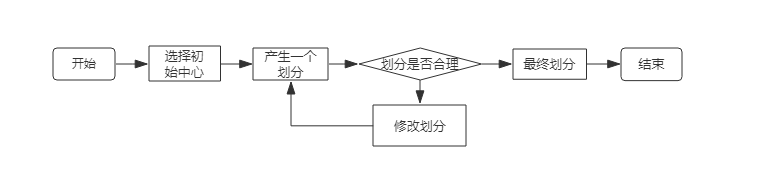
\includegraphics[width=1.0\linewidth]{Wsuanfaliuchengtu.png}
  \caption{算法流程图}
\end{figure}





\subsection{算法步骤}

$K-means$算法采用了贪心算法的思想,以迭代的方式对聚类结果进行更新,
最终获得最小的$SSE$.从某种角度来说,$K-means$算法是$EM$算法的一种特例,
两者的思想都是先固定一个变量然后在对另一个变量进行更新,如此反复直到收敛.
算法4.3给出了$K-means$算法的具体步骤: 

  

\begin{algorithm}[htb]
  \caption{ $K-means$}   
  \label{alg:Framwork}   
  \begin{algorithmic}[1] %这个1 表示每一行都显示数字  
  \REQUIRE ~~\\ %算法的输入参数:Input  
  All the set of point, $A$;\\  
  The number of clusters, $k$.\\   
  \ENSURE ~~\\ %算法的输出:Output  
  $k$ cluster center points.\\
  \STATE Randomly select k initial center points;    
  \STATE  \textbf{repeat} 
  \STATE \ \ \ \ Calculate the distance between each point and its own center point; \\
  \STATE \ \ \ \ Assign the points to other clusters with the closest distance to your center;
  \STATE \ \ \ \ By formula (4-5) obtained $c_k$, update the cluster center point;
  \STATE  \textbf{until}  The center point does not change;
  \RETURN $k$ coordinate. %算法的返回值  
  \end{algorithmic}  
\end{algorithm}  


\section{算法实现与分析}
\subsection{算法实现}
在$K-means$算法的实际执行过程中,
可能会出现已经进行了多次迭代而构成的簇还在发生变化的情况.
由于大部分的收敛都发生在早期阶段,在问题要求不是特别严格的情况下,
通常采用一种较弱的条件来替换算法的标准收敛条件,
例如“直到仅有1\%的点发生改变”,
这样弱化的收敛条件可以避免算法迭代次数过多的问题的发生,
在算法的精确性和时间效率上做出了一个平衡.算法执行构成如下图所示.

\begin{figure}[h!]
  \centering
  \begin{subfigure}[b]{0.4\linewidth}
    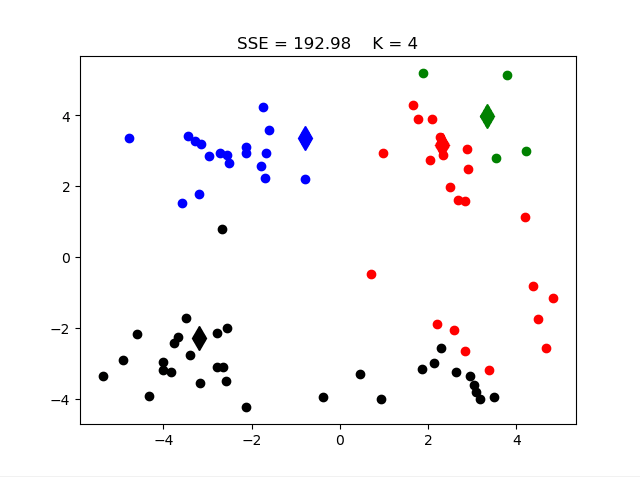
\includegraphics[width=\linewidth]{W4-1.png}
    \caption{第一次迭代}
  \end{subfigure}
  \begin{subfigure}[b]{0.4\linewidth}
    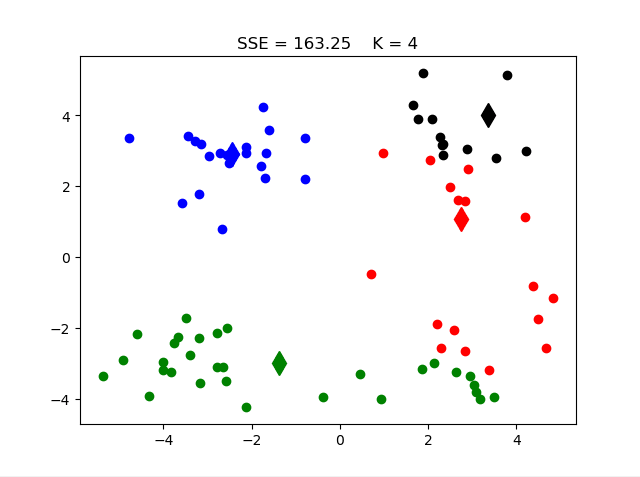
\includegraphics[width=\linewidth]{W4-2.png}
    \caption{第二次迭代}
  \end{subfigure}
  \begin{subfigure}[b]{0.4\linewidth}
    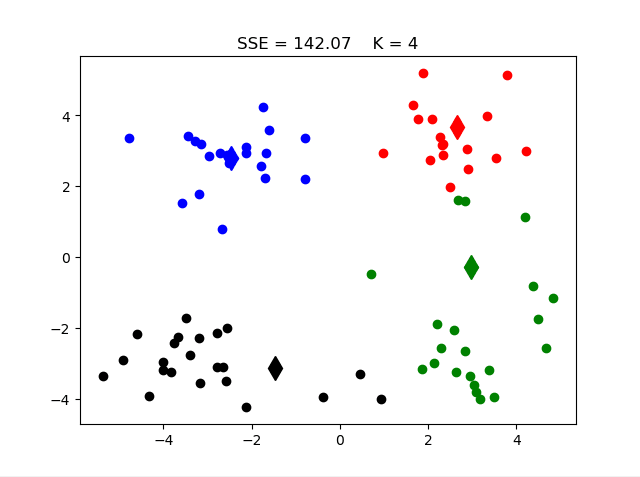
\includegraphics[width=\linewidth]{W4-3.png}
    \caption{第三次迭代}
  \end{subfigure}
  \begin{subfigure}[b]{0.4\linewidth}
    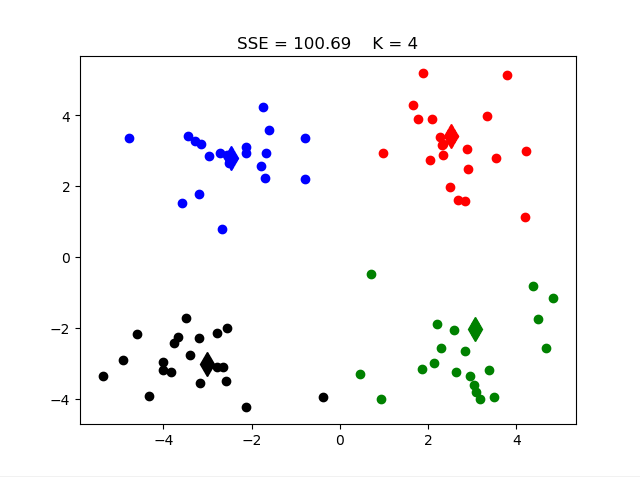
\includegraphics[width=\linewidth]{W4-4.png}
    \caption{第四次迭代}
  \end{subfigure}
  \begin{subfigure}[b]{0.4\linewidth}
    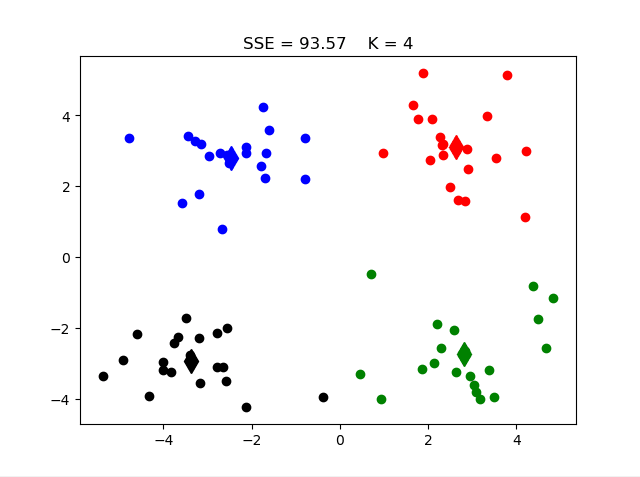
\includegraphics[width=\linewidth]{W4-5.png}
    \caption{第五次迭代}
  \end{subfigure}
  \begin{subfigure}[b]{0.4\linewidth}
    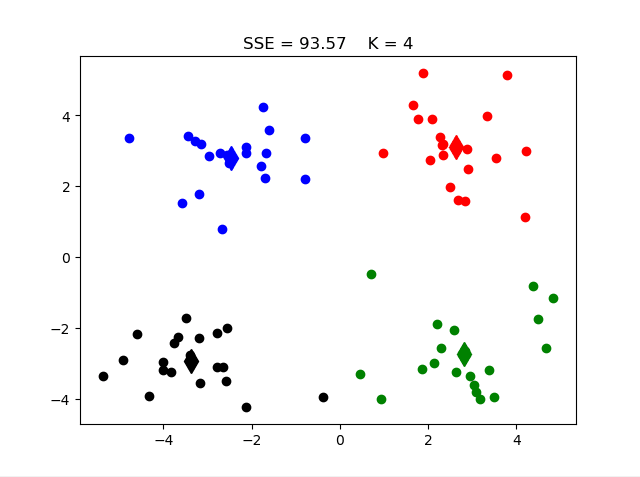
\includegraphics[width=\linewidth]{W4-6.png}
    \caption{第六次迭代}
  \end{subfigure}
  \caption{$K-means$算法执行过程}
\end{figure}

下面举例说明$K-means$算法是如何工作的.
如图4-3所示,数据集中一共包含四个类型的数据点,设定初始聚类个数为4.
首先,随机选取4个初始的中心点,即图中的钻石点.
接下来对于每个数据点,
计算它们与4个中心点的距离并选择最小的那个中心点,加入其表示的簇.
在是有数据点都分配完成后,计算每个簇中所有数据点的均值,
以此作为新的中心点,之后再次进行计算数据点与中心点之间的距离
来进行数据的重新分配,就形成了一次迭代后的数据分配.
重复进行分配和中心点更新这两个步骤,直至簇不在发生变化,
算法终止.如图4-3所示,(a)到(e)图中的中心点不点变化,
就是对中心点的不断更新,其中的有的数据点不断变化的颜色就是在进行重新分配,
直到(e)图,(e)图和(f)图是一样的,说明簇不在发生变化,算法终止.



\subsection{性能分析}
下面对$K-means$算法的性能进行分析,主要是对算法的时间复杂度和空间复杂度进行分析.
\begin{figure}[h!]
  \centering
  \begin{subfigure}[b]{0.8\linewidth}
    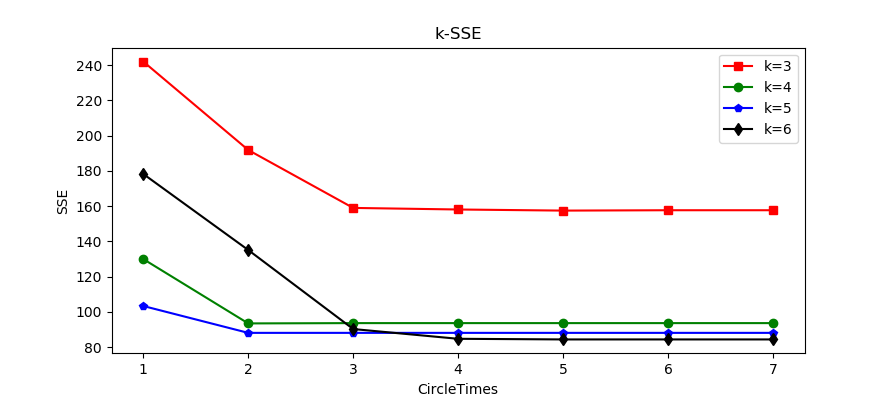
\includegraphics[width=\linewidth]{Wct-SSE-first.png}
    \caption{实验1 k-SSE迭代图}
  \end{subfigure}
  \begin{subfigure}[b]{0.8\linewidth}
    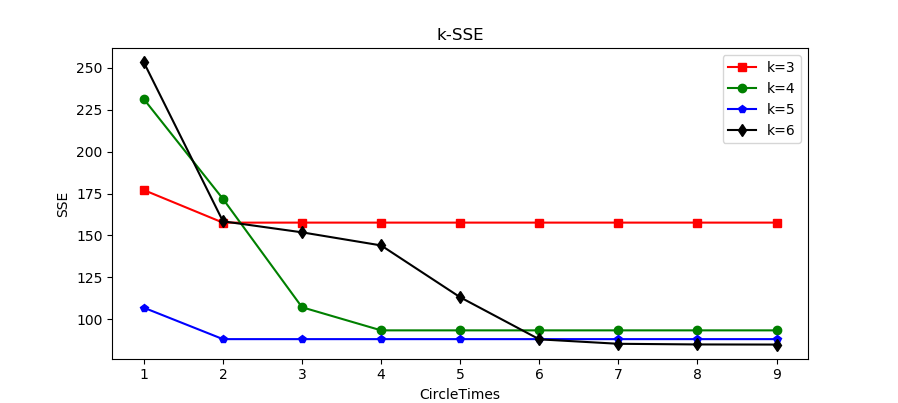
\includegraphics[width=\linewidth]{Wct-SSE-second.png}
    \caption{实验2 k-SSE迭代图}
  \end{subfigure}
  \caption{性能分析}
\end{figure}

在时间方面,$K-means$算法的时间需求基本上与数据点的个数成线性相关.
具体来说,其时间复杂度为$O(i*k*n*m)$,这里的$k$是簇的个数,
$i$是迭代次数(CircleTimes),n是数据集中包含数据点的个数,
m是每个数据的属性数.由于收敛大多发生在早期阶段,$i$的值通常比较小,
如上图所示,$i$为4就收敛了.这样,只要簇的个数$k$远小于$n$,
算法的计算时间就与$n$成线性相关.

在空间方面,$K-means$算法需要存放的类容只有数据点和每个簇的中心点数据.
具体来说,其空间复杂度为$O((k+n)*m)$,
这几个量的定义与计算时间复杂度时的定义一样.
一般可以认为,$i$,$k$和$m$都是常量.
这样的话,算法的时间复杂度和空间复杂度都可以简化为$O(n)$,即线性的.

由此可以看出,$K-means$是一种计算简单而又行至有效的聚类算法.

除了简单且有效以外,$K-means$算法还具有以下优点:

(1)算法使用于各种数据;

(2)当潜在的簇是凸的,
簇与簇之间大小相近且差异明显时,算法可以展现很好的聚类效果;

(3)对于大规模数据集合,该算法非常高效且伸缩性较好

但是,$K-means$算法还存在一些不足之处:

(1)首先,由于在中心点的更新步骤中,算法所使用的是簇内所包含的所有数据点的平均值.
如果在某一问题上无法定义簇内数据点的平均值,那么该算法无法发挥效果.
也就是说,该算法在处理具有分类属性的数据是就无从下手.

(2)在算法的初始化过程中,簇个数$k$的值和初始中心点的选取都对算法结果有着巨大的影响,
不合适的初始化值设定很容易造成算法最终收敛到局部最优值,这使得算法对先于知识具有较强的依赖性.

(3)算法对噪声点和离群点十分敏感,少量的异常数据就会对簇类平均值的计算造成巨大的干扰,
这种干扰很可能会造成簇划分不合理.

针对以上不足,我们可以从算法层面上对标准的$K-means$算法做出修改,
或是在初始化阶段完善对初始值的设定.
在接下来的的一节中,就改进初始化策略做出说明,提高了原有算法的性能,使算法具有更强的生命力.


\subsection{初始的选择}
对于$K-means$算法,有几个十分重要的因素影响着算法的聚类效果,
其中包括簇数目的选定、初始中心点的选取、距离度量的选择以及收敛条件的设定.
距离度量和收敛条件在本节之前已经说明过,余下两项就是在算法的最初阶段决定的,
这两个部分的初始化会直接影响最终能否得到合适的簇.


\begin{figure}[h!]
  \centering
  \begin{subfigure}[b]{0.4\linewidth}
    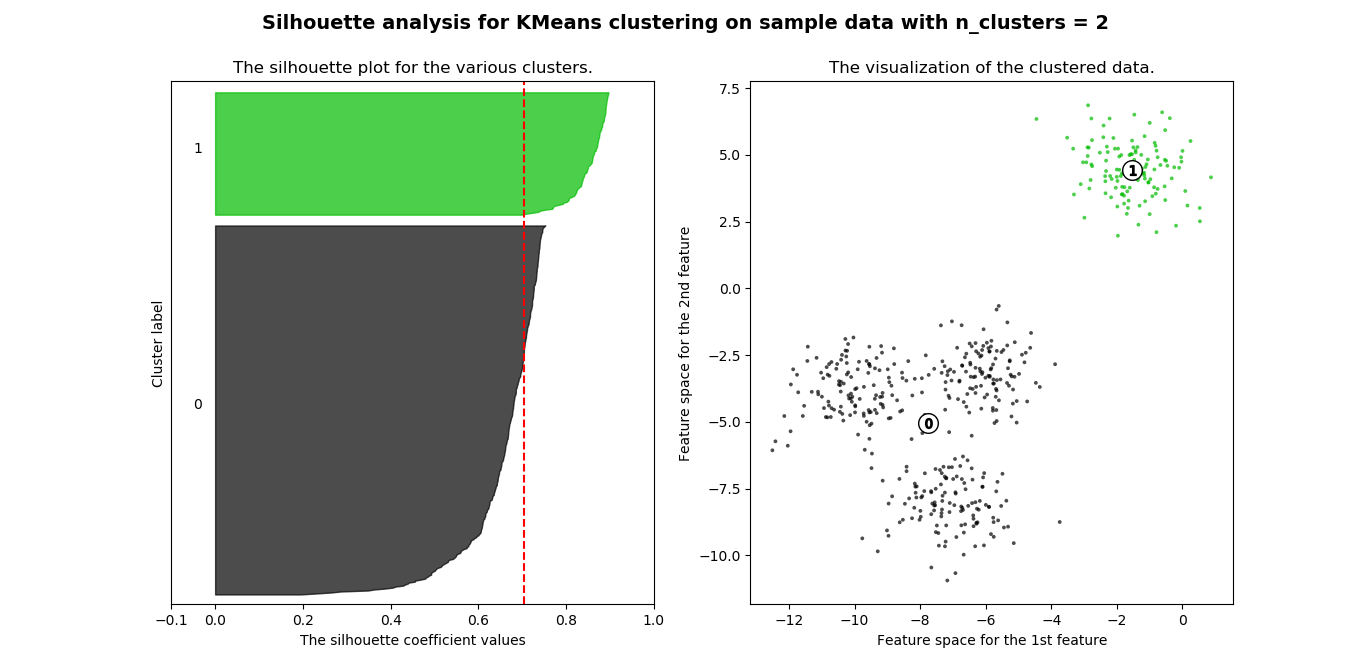
\includegraphics[width=\linewidth]{Wksh-2.png}
    \caption{k=2}
  \end{subfigure}
  \begin{subfigure}[b]{0.4\linewidth}
    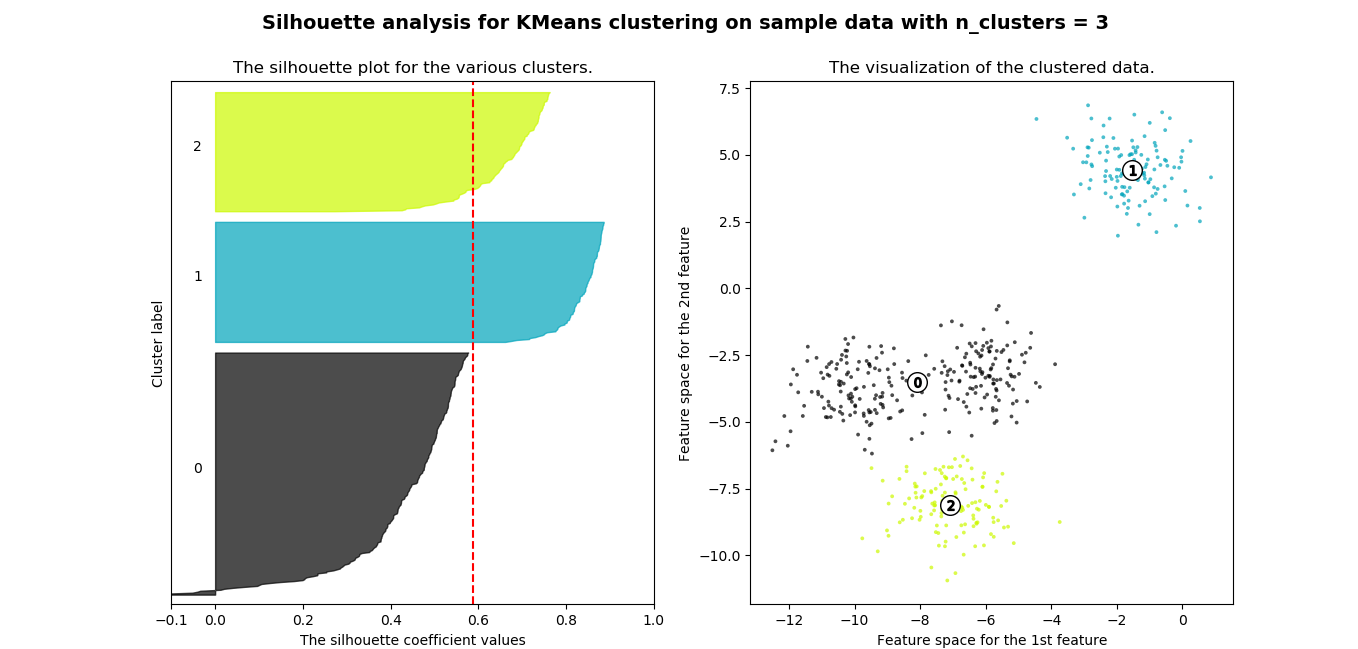
\includegraphics[width=\linewidth]{Wksh-3.png}
    \caption{k=3}
  \end{subfigure}
  \begin{subfigure}[b]{0.4\linewidth}
    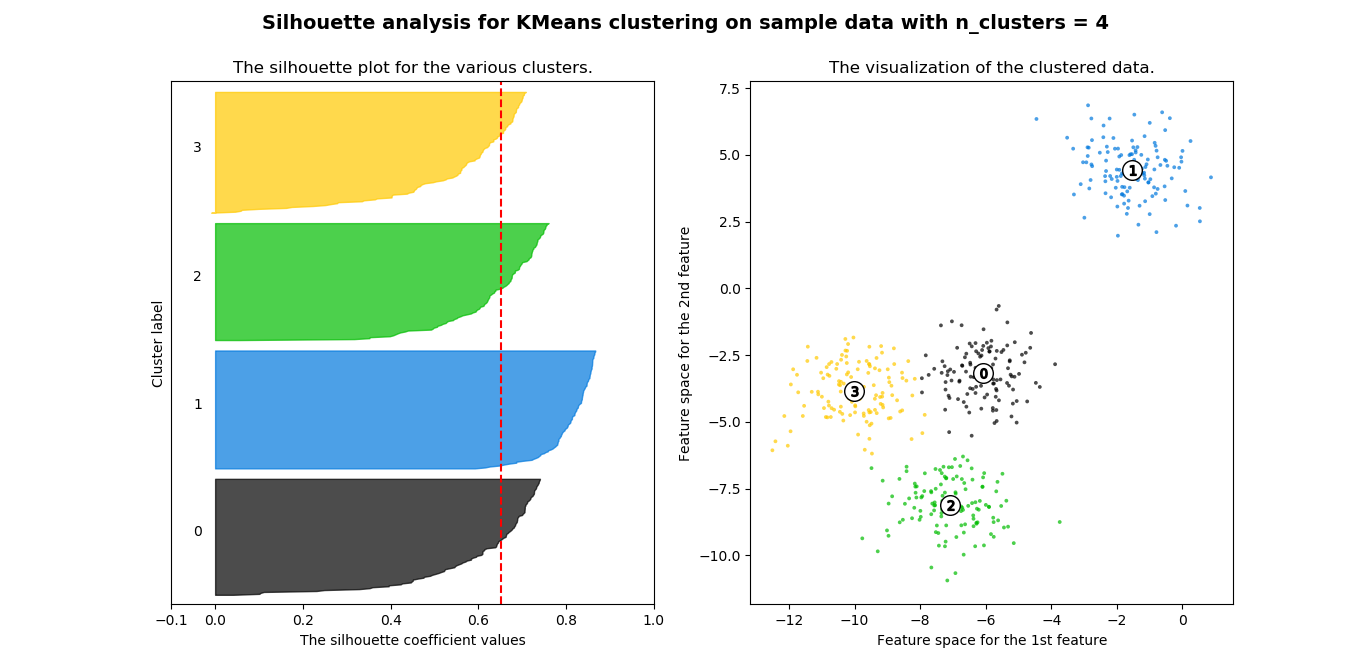
\includegraphics[width=\linewidth]{Wksh-4.png}
    \caption{k=4}
  \end{subfigure}
  \begin{subfigure}[b]{0.4\linewidth}
    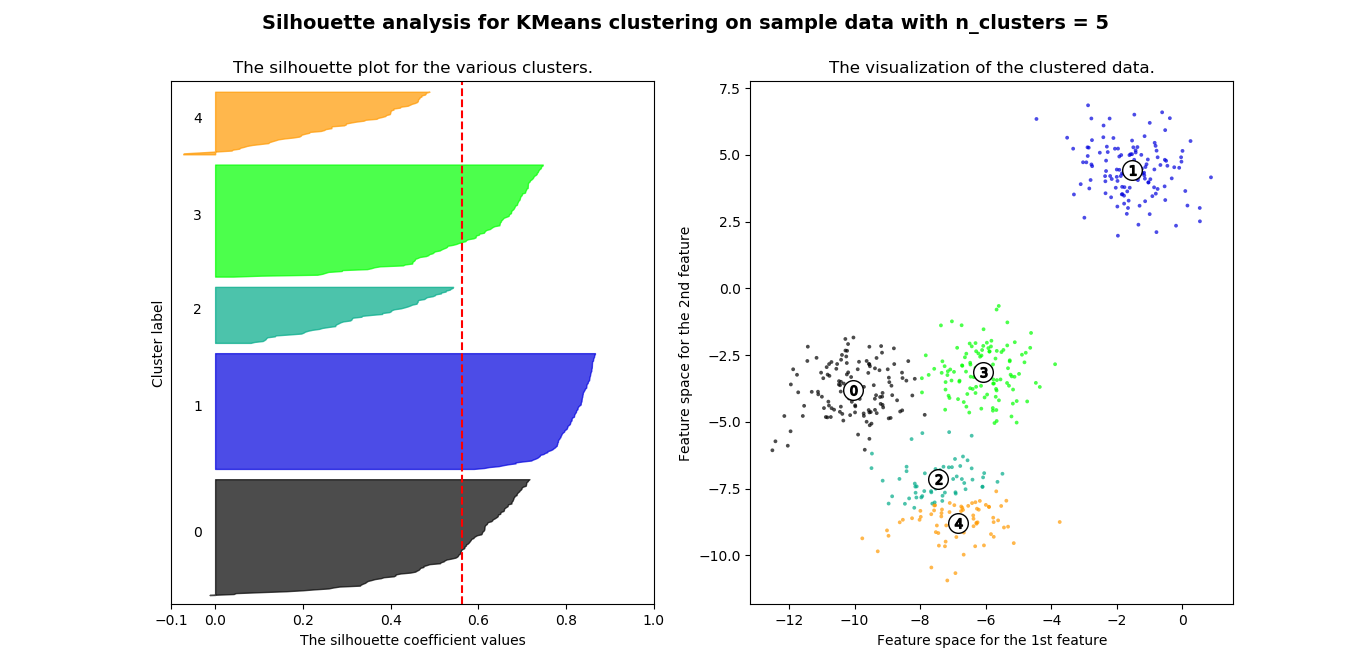
\includegraphics[width=\linewidth]{Wksh-5.png}
    \caption{k=5}
  \end{subfigure}
  \begin{subfigure}[b]{1.0\linewidth}
    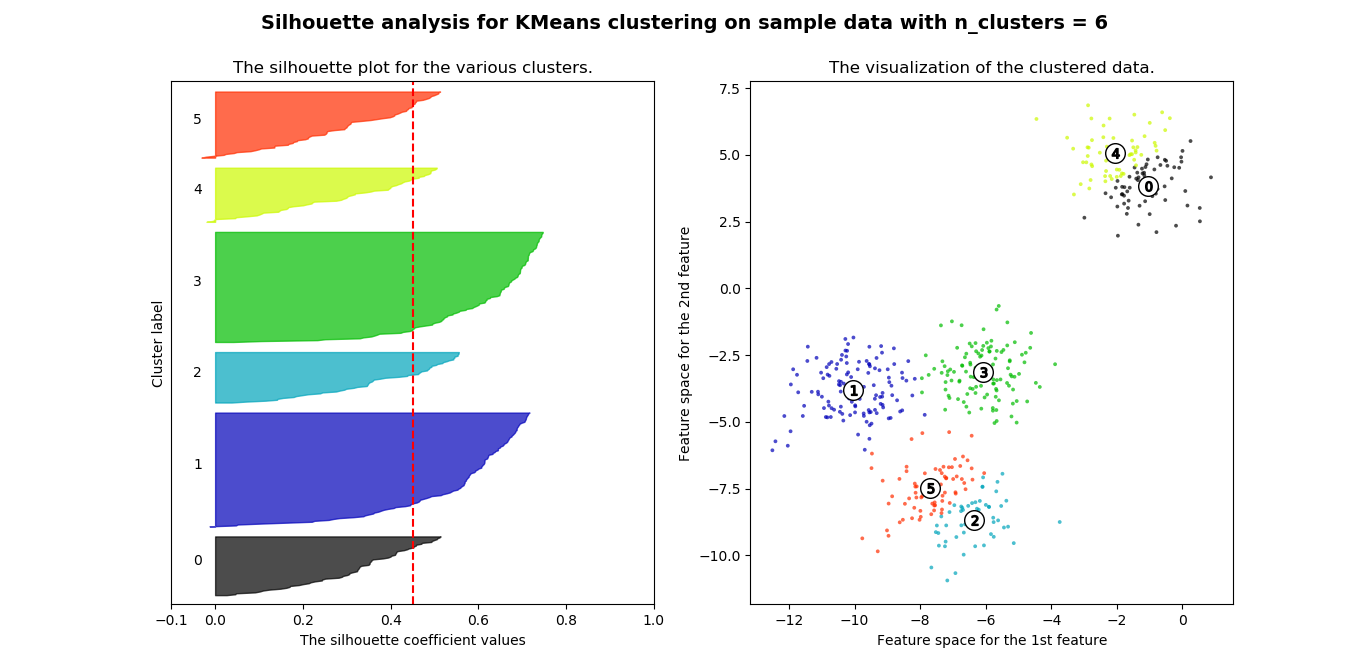
\includegraphics[width=\linewidth]{Wksh-6.png}
    \caption{k=6}
  \end{subfigure}
  \caption{数据可视化}
\end{figure}

$K-means$聚类算法最被人诟病的是类别个数k的选择,
这个设定往往会对结果造成很大的影响,为此提出了一种可行的方法.
该方法是设定一个最大阈值,
令k从小到大逐渐增加,观察SSE的变化从而选取合适的k.
因为k-均值算法中的目标函数是距离的平方和,随着k的增大,
每个簇的类别相似性也随之增加,由此造成SSE的变化是单调的减小.
如果以算法目标为基准,选取使SSE最小的k,
则当k取最大值,即k为数据集中数据个数的时候对应SSE最小.
但这样做是毫无意义的,因为每个数据对对象单独成一个簇.
这种变化来确定SSE的方法中,需要绘制k-SSE折线图,如图4.4所示.
观察图像,在最初k很小的时候,k的增大会使SSE的值迅速减小,之后趋于平缓.
因此,选取图像中的拐点附近的值作为k的起始值,就可以得到很好的聚类效果.


\begin{figure}[h!]
  \centering
    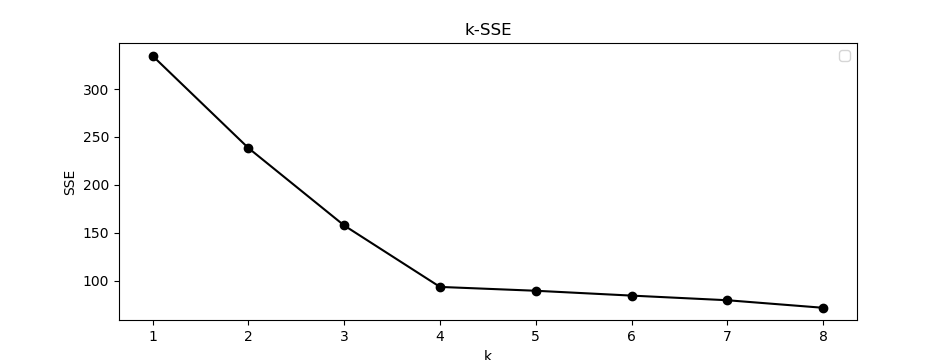
\includegraphics[width=0.8\linewidth]{Wk-SSE.png}
  \caption{k-SSE折线图}
\end{figure}



当然还有其他方法,如Calinski和Harabasz提出的Calinski-Harabasz指标、
Tibshirani等提出的计算差异量统计值方法、
赤池信息准则(akaike information criterion,AIC)、
贝叶斯信息准则(Bayesian information criterion,BIC)、
Newman和Girvan提出一种以结合层次聚类方法的k选取法、
Ball和Hall提出一种迭代自组织的数据分析算法——ISODATA等方法.
本文就不介绍了,有兴趣的话可以查阅相关资料.

上文介绍的是k值的选取,
还有一个重要选择的就是初始点的选择.
最基本的初始点的选取方式就是随机选取k个点作为初始中心点,
这是Macqueen提出的方法.
然而这种方法很容易造成算法最终陷入一个局部最优的解,所得到的聚类分布并不是最优的.
针对这样的问题,
本文采用的一种有效的方法就是选取初始点是先从数据集中随机抽取一些子样本集,
对每一个子样本及都实施随机选取初始中心点的$K-means$算法.
将算法运行后产生的中心点放到一个集合当中,构成一个仅由中心构成的集合,
对这一集合进行聚类分析,将的带的结果作为原数据集的初始中心点.



当然不只这一中有效方法,还有两种方法,一种是将$K-means$算法与聚合层次聚类方法相结合,
另一种是采用最近邻密度的观点.本文对这两种方法也不做详细的介绍.


\chapter{知乎用户的复杂网络研究}



\rule{\textwidth}{0.5pt}


\chapter{结论与展望}
\section{结论}
文本内容理解作为自然语言处理领域的一项核心技术,其研究在理论和实际应用
上都有重要的意义.
文本内容理解的主要任务是对序列建模,构建模型可以“学习”文本内在的表示特征.
当前基于RNN、LSTM等深度学习模型已经成为了主流方式,但是这种方式忽略了文本自身的语言学知识,
需要非常大的数据集而且缺乏可解释性和鲁棒性.

本文的主要工作是提出了融合依存句法结构的深度神经网络模型,并将模型运用的文本分类的具体应用上,
比传统的神经网络模型取得了更好的效果.

总的来说,通过文本分类的实验,可以看出融合模型具有下面几个优势:

(1) 因为融合模型学习了语言学知识,
所以在小规模数据集上融合模型的实验效果相对于RNN、LSTM模型有明显的提升,测试集上准确率提升3.1\%,
在大数据集上融合模型也具有有优势,测试集准确率最高提升2.5\%.

(2)通过引入Attention机制使得模型可以可视化出在
分类任务上文本中每一个子结构的重要程度,也就进一步可以可视化出
文本中的每一个单词的重要程度.通过可视化文本Attention的热力图,
使得模型具备一定的解释性.

(3)该模型引入依存句法作为语言学知识,
将融合模型的输出结果融合向量表示,可以送入后续任何形式的网络中,
来完成众多不同的文本理解任务.
并且该模型可以无缝替换原先的RNN、LSTM模型,因为融合模型和其输入输出形式完全相同,
所以可以很方便的升级原先的模型,将语言学知识引入原先的模型中.

本文还对模型的Attention方式和融合方式进行了深入的研究,实验表明
采用concatenation-based Attention和加权融合能产生最好的实验结果,
相对LSTM模型提升了2.5\%的准确率.

\section{不足与展望}
因为文本内容理解本身就是一件复杂的研究领域,所以由于条件和时间等方面的原因,
本文的方法还存在需要改进和完善的地方,主要如下:

(1)该模型目前仅仅在在文本分类的任务上进行了实验,还未在更多的文本内容理解任务上实验,
所以可能在某些其他任务上实验效果会不如人意.
尤其对于中文依存句法的解析效果目前还不如英语,所以本模型在处理中文语境下可能会较差,
当然这需要进一步实验来改进调整模型.

(2)该模型由两个独立的LSTM模型和依存句法解析工具构成,所以模型复杂度较高,
在在线处理文本上实时性相对于传统RNN、LSTM模型较差.
主要性能瓶颈在句法解析上,所以未来可能考虑将句法解析融入网络中,
或者引入性能更高的句法解析工具.


% 参考文献.应放在\backmatter之前.
% 推荐使用BibTeX,若不使用BibTeX时注释掉下面一句.
\nocite{*}
\bibliography{bachelor}
% 不使用 BibTeX
%\begin{thebibliography}{2}
%
%\bibitem{deng:01a}
%{邓建松,彭冉冉,陈长松}.
%\newblock {\em \LaTeXe{}科技排版指南}.
%\newblock 科学出版社,书号:7-03-009239-2/TP.1516, 北京, 2001.
%
%\bibitem{wang:00a}
%王磊.
%\newblock {\em \LaTeXe{}插图指南}.
%\newblock 2000.
%\end{thebibliography}

%%%%%%%%%%%%%%%%%%%%%%%%%%%%%%%%%%%%%%%%%%%%%%%%%%%%%%%%%%%%%%%%%%%%%%%%%%%%%%%
% 致谢,应放在《结论》之后
\begin{acknowledgement}
感谢我的毕设导师王澜老师,感谢他在毕设的各个环节对我的提醒、检查和督促.

感谢我的研究生导师黄河燕教授,她让我在本科的最后阶段
接触到了自然语言处理这个领域,并给我提供了开放自由的科研环境,以及对我毕设全程的关心和指导.

还要特别感谢魏骁驰博士,他学识渊博,毕设的从始至终一直一步步指导我完成,
耐心解答了我所有提出的问题.帮助我明晰了每一步需要做什么,具体怎么做,做好了如何完善.
将原本很难的课题,分解成一个个小问题,指导我去解决.
并且他在工作中认真负责,在生活中积极开朗的性格也深深的感染了我.

感谢所有任课老师孜孜不倦地教导,让我在大学四年学到了方方面面的知识.
感谢我的班主任冯伟老师,是他引导我走上科创的道路,并认识了很多优秀的同学.

感谢我的家人,感谢他们对我的无私奉献,是我一直以来的坚强后盾,
帮助我一起面对困难,战胜困难.

最后,真挚的感谢所有给我提供帮助和鼓励的人.
\end{acknowledgement}

\backmatter




%%%%%%%%%%%%%%%%%%%%%%%%%%%%%%%%%%%%%%%%%%%%%%%%%%%%%%%%%%%%%%%%%%%%%%%%%%%%%%%
\end{document}
